% Manuscript: Predictive latent dynamics for parametric vortex-gust airfoil
% interactions at Re = 5000.
% Build: pdflatex main && bibtex main && pdflatex main && pdflatex main
% Target venue: J. Fluid Mech. (Rapids-adjacent length) / Phys. Rev. Fluids.
%
% ----------------------------------------------------------------------------
% REWRITE NOTE (read REWRITE_NOTES.md first):
% This is a structural and stylistic rewrite of the original eight-section draft
% into the six-section idiom of the Taira-group extreme-aerodynamics literature
% (Smith et al. 2024 JFM; Fukami, Nakao & Taira 2024 JFM; Fukami & Taira 2025 JFM;
% Tran, Yeh & Taira 2026 JFM; Odaka, Lopez-Doriga & Taira 2026 JFM). It removes
% the implementation diary, demotes the SIGReg-vs-PLDM material to a single
% methods paragraph plus an appendix, and reframes the headline onto held-out
% evidence. Claims that require the not-yet-run controls are marked inline with
% % PENDING. New analyses adapted from the references are scaffolded with their
% method text written and their results marked % RESULT PENDING.
% ----------------------------------------------------------------------------

\documentclass[11pt,a4paper]{article}

\usepackage[utf8]{inputenc}
\usepackage[T1]{fontenc}
\usepackage{lmodern}
\usepackage[margin=1in]{geometry}
\usepackage{amsmath,amssymb,amsfonts}
\usepackage{graphicx}
\usepackage{booktabs}
\usepackage{longtable}
\usepackage{xcolor}
\usepackage{hyperref}
\usepackage{caption}
\usepackage{subcaption}
\usepackage{authblk}
\usepackage{microtype}
\usepackage{enumitem}

% Lightweight TODO macro so pending items are visible in the compiled PDF.
% Set \pendingon to \pendingoff before submission to hide them.
\newcommand{\pending}[1]{{\color{red}\textbf{[PENDING: #1]}}}

\hypersetup{
  colorlinks=true,
  linkcolor=blue!50!black,
  citecolor=blue!50!black,
  urlcolor=blue!50!black
}

\title{Forward physical closure of predictive and reconstructive latents for
vortex-gust airfoil interactions at $\mathrm{Re}=5000$}
\author[1,2]{Alberto Solera-Rico}
\author[3,4]{Arnau Mir\'o}
\author[4]{Oriol Lehmkuhl}
\author[1,2]{Carlos Sanmiguel Vila\thanks{Corresponding author: \texttt{csanvil@inta.es}}}
\affil[1]{Aerial Platforms Department, Spanish National Institute for Aerospace Technology (INTA), ROR: \url{https://ror.org/02m44ak47}, San Mart\'in de la Vega, 28330, Madrid, Spain}
\affil[2]{Department of Aerospace Engineering, Universidad Carlos III de Madrid, ROR: \url{https://ror.org/03ths8210}, Legan\'es, 28911, Madrid, Spain}
\affil[3]{TUAREG Research Group, Universitat Polit\`ecnica de Catalunya (UPC), Carrer Colom 11, 08222 Terrassa, Spain}
\affil[4]{Barcelona Supercomputing Centre (BSC), CASE Large-Scale Computational Fluid Dynamics, Pla\c{c}a d'Eusebi G\"uell, 1-3, 08034 Barcelona, Spain}
\date{}

\newcommand{\vRe}{\mathrm{Re}}
\newcommand{\zvec}{\mathbf{z}}
\newcommand{\xvec}{\mathbf{x}}
\newcommand{\cvec}{\mathbf{c}}
\newcommand{\uvec}{\mathbf{u}}
\newcommand{\omegaz}{\omega_z}

\begin{document}

\maketitle

\begin{abstract}
% Abstract, bound from editorial/upstream/front_matter_rewrite.tex at the
% Session 37 Stage 4 front-matter bind (author-approved, D303/D306) and
% trimmed to the 250-word gate at Session 38 per Carlos's instruction
% (2026-07-11): micro-trims only, no content removed.
% REVIEW-CLAIM: (Session 38) "the predictive coordinates are the most
% forecastable" corrected to "the wake-supervised states are the most
% forecastable": the D310 shared-operator recomputation makes the top block
% a statistical tie among the wake-headed states, so the draft's sentence
% (written pre-M1) is no longer supportable as stated.
Extreme vortex gusts drive a post-stall airfoil through a transient
reorganisation of its wake, and the release parameters alone do not
determine the flow after the vortex passes. We ask whether a reduced
state of the encounter can retain the wake dynamics, remain usable
under a low-order forecast model, and be estimated from the sparse wall
pressure a wing can carry. We compare predictive, reconstruction-trained
and proper-orthogonal-decomposition coefficient states at matched
dimension, on direct numerical simulations of a NACA 0012 airfoil at
$\alpha = 14^\circ$ and $\vRe = 5000$ perturbed by Taylor vortices
spanning gust ratio, core diameter and offset. A controlled supervision
study shows different ingredients supply the requirements.
Under the predictive objective considered, a scalar lift target is
necessary against latent collapse, a near-body force-element target
sharpens the peak loads, and a wake target is required for the wake
enstrophy and circulation; the multi-step predictive objective
contributes rollout stability rather than instantaneous readability.
Load information remains accessible at four coefficients, whereas
wake-field reconstruction requires at least sixteen. Under one
\DirectFC{} trained identically on every state, the wake-supervised
states are the most forecastable, autoregressive rollout degrades
through error accumulation, and supplying the true gust parameters
provides no benefit. A sequential ensemble filter sensing eight
wall-pressure taps then tracks the lift through the encounter, with
impact-phase $R^2 = \PoneTwoStageCovImpact$ (root-mean-square error
$\PoneTwoStageCovRmse$ in lift units) on the \TestSplit{} set and
$\PoneTwoStageCovImpactC$ at the held-out $|G| = 4$ boundary; the wake
enstrophy is not recovered by the wall-sensor configurations considered,
a limit of the sensing geometry rather than the state.

\end{abstract}

\noindent\textit{Key words:} vortex shedding, low-dimensional models, machine learning

\section{Introduction}
\label{sec:introduction}
% Introduction. Related work (former Section 2) is folded in here, in the JFM
% idiom (no standalone "Related work" section). The SIGReg-vs-PLDM "second paper"
% that headed Section 1.2 of the original draft has been removed; the regulariser
% choice is now a methods detail (Sec. 3) and an appendix. Reframed 2026-06-08 for
% the fully UNCONDITIONED model: no gust parameters enter the encoder or the
% predictor. Contributions are reframed around the representational wake closure
% the predictive objective produces, with the rollout shown but not headlined as
% forward closure, and the world-model reading kept as motivation only.

A discrete vortex gust striking a post-stall airfoil does not merely perturb the
force coefficients: it reorganises the separated wake. The lift excursion it
produces is the surface signature of leading-edge-vortex roll-up, growth, and
shedding, the dominant unsteady mechanism in these encounters
\citep{eldredge2019leading}, together with the trailing-edge and wake structures
it leaves behind, and it is set by the timing of the vortex impact relative to the
airfoil's own shedding, the wall-normal offset of the vortex core, and the gust
strength and core size. Such extreme gusts arise wherever the gust velocity is
comparable to or larger than the flight speed, for small uncrewed and micro air
vehicles in urban canyons, mountainous terrain, and the wakes of buildings and
ships \citep{jones2022,mohamed2023gusts}: the gust ratio $G$, the ratio of the
characteristic gust velocity to the free-stream velocity, then exceeds unity, and
conventional gust models do not capture the resulting large, fast load transients
\citep{fukami2024control,fukami2025prf}. Even at the moderate chord Reynolds number
$\vRe = 5000$, the post-stall flow at $\alpha = 14^\circ$ is massively
separated, and the gust-induced disturbance interacts nonlinearly with the
natural shedding cycle \citep{fukami2025prf}; the vortical organisation of the
encounter is moreover similar across laminar and turbulent regimes
\citep{odaka2026}, so this case is representative of the wider extreme-aerodynamic
family. Resolving the full parametric
envelope by simulation is expensive, so reduced-order models (ROMs) of the
encounter-to-encounter and case-to-case variability are an active line of work.
A reduced model for such an encounter must do more than reproduce a vorticity
snapshot or the instantaneous force: it must retain the wake variables that
determine the post-impact transient and organise them into a state on which a
forward model can be queried without leaving the data manifold. This is the
predictive-state problem that organises the present study.

Reduced-order models of such flows form a ladder of increasing nonlinearity.
Energy-optimal linear bases, proper orthogonal decomposition
\citep{berkooz1993pod} and dynamic mode decomposition \citep{schmid2010dmd}, are
compact and interpretable but limited for strongly nonlinear separation; their
Koopman-operator reading \citep{lusch2018deep} nonetheless makes a linear latent a
principled comparator rather than a strawman. Nonlinear autoencoders compress
further at matched latent dimension \citep{murata2020nonlinear,lee2020model}, and
coupling an
autoencoder to a learned latent dynamics forecasts better than dynamics confined
to a linear subspace \citep{linot2023dynamics}. Read as a design ladder, these
methods progress from field reconstruction and energy compression, through
observable readability, toward forward-state usability, which is the property a
reduced state needs to serve a predictor; the extreme-aerodynamic reduced models we
build on sit at the nonlinear, observable-augmented rung, and the question we pursue
is what carries a state the rest of the way.

Recent ROMs for separated and extreme-aerodynamic flows, increasingly built with
machine learning \citep{brunton2020machine}, share a common
ingredient: a reconstruction-trained autoencoder whose bottleneck is shaped by
an auxiliary aerodynamic observable. Fukami \& Taira \citeyearpar{fukami2023} trained
a convolutional autoencoder jointly with a lift-prediction head and found that
the auxiliary loss reduced the intrinsic dimension of the discovered manifold
for extreme vortex-gust flows from roughly ten to three. The same
observable-augmentation idea was extended across multi-source turbulent data
\citep{fukami2025}, and was used by Solera-Rico et al. \citeyearpar{solera2024} with a
$\beta$-variational autoencoder and a transformer ROM on a vortex-gust airfoil
dataset of the same family considered here. Across this lineage the
reconstruction term anchors the latent geometry to the instantaneous flow
field, and an observable-prediction term orients it along aerodynamically
relevant directions. A recurring theme of the geometric-analysis literature,
however, is that the latent coordinates of an autoencoder are unique only up to
a diffeomorphism, so reconstruction leaves the geometry of the latent largely
unconstrained, which complicates any downstream task that relies on that
geometry, including dynamics, interpolation, and comparison
\citep{tran2026,kelshaw2024}. Observable augmentation solves only one part of the
predictive-state problem: it tells the encoder which aerodynamic quantity to
represent, but it does not by itself fix whether the latent coordinates are
suitable for time advancement. A reduced state that is linearly readable at a single
instant may still be unusable once an autoregressive predictor queries the points
its own rollout produces.

A parallel and fast-growing line reads these flows through the information their
reduced states carry rather than their energy. Transfer-entropy causality among
proper-orthogonal-decomposition modes ranks which modes drive the formation of
coherent structures \citep{martinezsanchez2023}, and an informative/non-informative
decomposition splits a field into the part that carries information about a
target's future and a residual that carries none \citep{arranz2024}. This
informative-decomposition idea has very recently been brought to extreme
vortex-gust airfoil interactions of the present family, extracting the field
structures informative about the future lift \citep{koshikawa2026,fukamiaraki2026},
alongside time-dependent modal bases for the same interaction
\citep{zhong2025,zamaniashtiani2025} and latent-causality attributions in physical
space \citep{cremades2026xcal}. Our study is complementary: rather than mapping the
informative or causal modes of a single representation, we ask which encoder
objective produces a latent whose forward evolution closes the full set of
observables, the wake included, and we use the information lens only as a held-out
diagnostic of the resulting latent (\S\ref{sec:disc_mechanism}).

A complementary route to a reduced state is to drop the reconstruction term
altogether and to train the encoder and a predictor end to end on
latent-space forecasting, with an explicit anti-collapse regulariser in place
of the decoder. This is the joint-embedding predictive architecture (JEPA)
\citep{lecun2022}: an encoder maps the input to a representation, a predictor
advances that representation in time, and the loss never reconstructs the
field. The encoder is thereby trained in the same coordinates in which the
predictor will later operate, which makes JEPA a useful instrument for testing
whether predictive training produces a latent state that remains usable when rolled
forward, rather than merely readable when encoded from the DNS field; the predictor
also cannot exploit pixel-level shortcuts, because no field-space signal reaches it. The image and video
instantiations \citep{ijepa,vjepa2} and the recent from-pixels variants that
remove the moving-target encoder in favour of a characteristic-function
regulariser \citep{lewm,lejepa} or a variance-covariance objective
\citep{pldm,vicreg} have so far been evaluated on gridworld and toy visual
domains. Their behaviour on a low-intrinsic-dimension physics dataset, where
the data sit on a roughly five- to ten-dimensional manifold, is uncharacterised.

Reconstruction-trained nonlinear encoders compress aggressively but yield latent
dynamics that are harder to forecast than an energy-optimal linear basis, a
compactness-versus-forecast tradeoff documented for controlled wake flows in a
companion study under review \citep{solerarico_compactness_underreview}. We show
this tradeoff is a consequence of the reconstruction objective: a predictive
latent recovers nonlinear compactness without surrendering forecast stability.
The division of labour with that companion study
\citep{solerarico_compactness_underreview} is explicit: there, controlled
canonical wakes and the compactness-versus-forecast tradeoff; here, the
parametric vortex gust, the latent-drift mechanism we identify as the common
cure, and its geometric and topological characterisation.

The model we adopt takes no gust parameters: $(G, D, Y)$ enter neither the encoder
nor the predictor. The encoder is a pure state map and the predictor advances the
latent from its own history alone. The world-model framework of
\citet{lecun2022,ha2018world} motivates this split as an analogy and not a property
we claim, since the latent dynamics function is the object a controller would plan
against, and a recent gust-airfoil instance couples a physics-augmented autoencoder
to a latent dynamics model \citep{liu2025modelbased}. We treat that reading as
motivation: the rollout is shown as a consistent latent trajectory rather than
advanced as a validated forecast, and its interventional or causal interpretation is
left for future work (\S\ref{sec:discussion}). What this leaves is the
property our study turns on: an established reconstruction-trained autoencoder and an
energy-optimal proper orthogonal decomposition basis, lacking wake supervision, do
not keep the dynamically relevant wake observables linearly readable, and even a
wake-readable state is not automatically usable once a forward model advances it.
The drift mechanism of \S\ref{sec:res_drift} and the division of labour we identify
are the empirical consequences.

The question this paper addresses is therefore not which encoder reconstructs
the flow best, nor even which produces a reduced state from which the wake is
readable at a single instant, but which produces a state that is also usable once a
forward model advances it. We treat this as a fluid-mechanics question with a
geometric answer, and find a division of labour: wake-observable supervision makes
the wake readable, an anti-collapse regulariser keeps the latent in distribution
under rollout, and the predictive objective makes the supervised state dynamically
trackable. The joint-embedding predictive architecture is the instrument we use to
test this principle, not the subject of the paper. We make three contributions.

First, we formulate the vortex-gust encounter as a predictive-state benchmark. The
primary endpoint is the wake enstrophy at a fixed post-impact readout ($H = 16$),
because it summarises the leading-edge-vortex roll-up and wake reorganisation that
the scalar force can miss; all encoders, a predictive one (JEPA), a reconstructive
one in the Fukami lineage, and a POD basis, are compared at matched latent dimension
under a single shared probe and autoregressive predictor (\S\ref{sec:methods}). The
question is then not field-reconstruction quality but whether the reduced state
carries the wake variables a forward model needs (\S\ref{sec:res_closure}).

Second, we separate the ingredients of a usable predictive state
(\S\ref{sec:res_controls}). Wake-observable supervision supplies the instantaneous
readability: on held-out fields the wake-supervised states make the wake enstrophy
linearly readable ($R^2 = \NumReprWakeJepaTf$) where the no-wake reconstructive and
linear baselines are at or below zero, but an objective-free supervised encoder
reads it as well, and a matched reconstructive control reads it comparably once
retrained out of sample, so the readability is the supervision's, not the
objective's. Anti-collapse regularisation supplies an in-distribution geometry: the
supervision-only and predictive rollouts both stay on the encoded manifold, where
the reconstructive rollout departs along directions of negligible encoded variance
(\S\ref{sec:res_drift}). The predictive objective supplies the dynamic usability: its
rollout stays closer to the encoded simulation trajectory and forecasts the wake
better than the objective-free and reconstructive alternatives.

Third, we interpret the resulting state physically and observationally
(\S\ref{sec:res_flow_physics}, \S\ref{sec:res_observability}). The predictive state
keeps the undisturbed shedding orbit as a single loop under a metric that removes
coordinate scale, carries the wake response across the tested readout horizons, and
is the most recoverable of the three from sparse pre-impact wall pressure. These
results motivate the state as an input to a future estimator or controller; the
present paper does not claim a validated forecast or a closed-loop controller.


\section{Flow configuration and data}
\label{sec:flow}
% Flow configuration and data. New physics-first section in the idiom of
% Fukami's "Flow physics" subsection and the PRF "Simulation setup". It (i)
% describes the encounter as a staged cycle (base -> LEV -> arch/TEV -> recovery),
% following Smith et al. 2024 and Odaka et al. 2026; (ii) frames the baseline as
% a limit cycle, following Fukami, Nakao & Taira 2024; (iii) reframes |G|=4 as a
% physical 2D->3D regime change, following the PRF source paper; (iv) defines the
% six observables physically. The implementation-diary split metadata, the sha,
% and the hardware lines from the original Methods are removed.

\subsection{Vortex gust-airfoil interaction}
\label{sec:flow_physics}

\rb{K}{S2-01}{Configuration, solver provenance and the gust parametrisation. The DNS-not-LES and Fukami-as-reference-not-source distinctions live here.}We study a NACA~0012 airfoil at angle of attack $\alpha = 14^\circ$ and chord
Reynolds number $\vRe = 5000$, perturbed by a discrete vortex gust modelled as a
spanwise-oriented Taylor vortex released upstream of the leading edge. The data
analysed here are our own direct numerical simulations of this configuration,
computed with the GPU-enabled spectral-element solver SOD2D
\citep{gasparino2024sod2d} with no subgrid-scale model, so that all scales of the
separated wake are resolved at this Reynolds number. The solver uses an
incompressible, constant-density pressure-projection formulation
($M = 0$; table~\ref{tab:dns_pending}). The configuration and its physical characterisation follow
Fukami, Smith \& Taira \citeyearpar{fukami2025prf}, which is the reference for the
physics, not the source of the data.
The vortex has the azimuthal velocity profile
\begin{equation}
  u_\theta(r) = u_{\theta,\max}\,\frac{r}{R}\,
  \exp\!\left[\tfrac12\!\left(1 - \frac{r^2}{R^2}\right)\right],
  \label{eq:taylor}
\end{equation}
which peaks at the core radius $r = R$ \citep{taylor1918}, and is parametrised by
three scalars: the signed gust ratio $G \equiv u_{\theta,\max}/u_\infty$, the
core diameter $D \equiv 2R/c$, and the offset $Y$ of the vortex centre,
measured normal to the free stream (figure~\ref{fig:geometry}). The release
point is fixed at $2c$ upstream of the leading edge and offset by $Y$, both
measured in axes aligned with the free stream, following
\citet{fukami2025prf} and the chord is pitched by the angle of attack $\alpha$
relative to these axes. The profile and the $(G, D, Y)$
sampling follow the configuration of \citet{fukami2025prf}. The training envelope spans $|G| \in \{0.25, 0.5, 1.0, 1.5, 2.0,
3.0\}$ with $G = 0$ as the undisturbed reference, $D \in \{0.5, 1.0, 1.5\}$
chords, and $Y \in [-0.4, +0.4]$; the value $|G| = 4$ is held out as an
extrapolation boundary, for reasons that are physical and that we return to
below. Convective time $t$ is measured in chords from the vortex release,
$t = 0$, while $t_{\mathrm{imp}}$ denotes the instant at which the vortex centre
reaches the leading edge, near $t/c = 2$ for this configuration; all phase
windows below are referred to $t_{\mathrm{imp}}$.\re

\begin{figure}
  \centering
  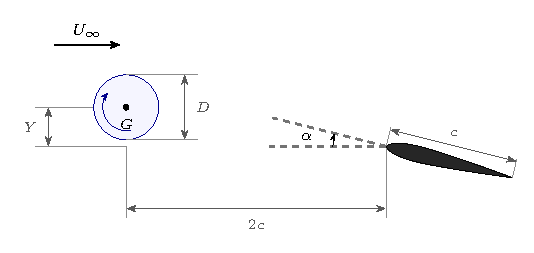
\includegraphics[width=\linewidth]{sections/figures/tikz/fig_case_geometry.pdf}
  \caption{\rb{K}{S2-C1}{Defines the free-stream-aligned axes in which $(G,D,Y)$ are read. Without it the sign conventions of the envelope result are ambiguous.}Case geometry (schematic, not to scale), drawn directly in the
  free-stream-aligned axes in which $(G, D, Y)$ are defined, following
  \citet{fukami2025prf}. The vortex core is released a fixed $2c$ upstream of
  the leading edge (LE), offset by $Y$ normal to the free stream $U_\infty$,
  and convects downstream parallel to it, not along the chord. The chord is
  pitched by the angle of attack $\alpha = 14^\circ$ relative to these axes,
  trailing edge (TE) below leading edge. The core has diameter $D = 2R/c$
  (core radius $R$) and peak azimuthal velocity $u_{\theta,\max}$ setting the
  signed gust ratio $G \equiv u_{\theta,\max}/u_\infty$; the arrow shows the
  clockwise sense of rotation for $G > 0$. Only $(G, D, Y)$ vary across cases.\re}
  \label{fig:geometry}
\end{figure}

\rb{K}{S2-02}{The staged reading of the encounter that the five observables summarise. Physics framing the Results repeatedly refer back to.}Without a gust, the $\alpha = 14^\circ$ wake at this Reynolds number is separated and sheds periodically; in dynamical terms the undisturbed
flow is a limit cycle. A gust encounter is then a transient excursion from this
limit cycle and back, and it is helpful to read it in stages
(figure~\ref{fig:staging}) \citep{smith2024,fukami2025prf,odaka2026}. The vortex
first induces a strong
wall-normal vorticity flux at the leading edge, the airfoil experiences a sharp
lift excursion as a leading-edge vortex (LEV) forms, the LEV rolls up and sheds
together with a trailing-edge structure as the load reaches its extremum, and
the wake then relaxes back toward the baseline shedding. The sign of $G$ sets
whether the first lift excursion is positive or negative, $Y$ sets the side and
strength of the impingement, $D$ sets how much of the encounter is dominated by
the vortex core, and the impact timing sets the phase of the baseline cycle at
which the disturbance arrives. The five observables defined in
\S\ref{sec:flow_observables} are quantitative summaries of exactly this
sequence.\re

\begin{figure}
  \centering
  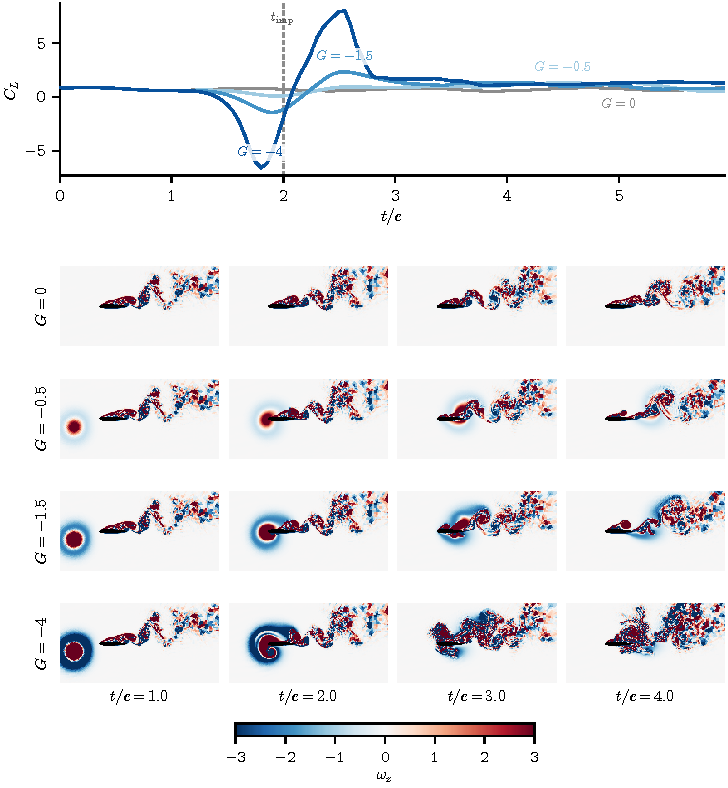
\includegraphics[width=\linewidth]{sections/figures/results/fig_staging_v2p1.pdf}
  \caption{\rb{K}{S2-C2}{The gust-strength sweep that shows the wake reorganisation the paper is about. Also states why the wake, not only $C_L$, is the endpoint.}The vortex gust as a wake-reorganisation event: a gust-strength sweep
  at fixed core diameter $D = 0.5$ and offset $Y = -0.1$ (first encounter of each
  case). Top: lift coefficient $C_L$ against convective time, with $t/c = 0$ the
  release and $t_{\mathrm{imp}}$ (dashed) the leading-edge crossing near
  $t/c = 2$; the load excursion deepens and widens with $|G|$, the baseline
  ($G = 0$) in grey. Bottom: mid-plane spanwise vorticity $\omegaz$ per case (rows
  $G = 0$, $-0.5$, $-1.5$, $-4$) at four times (columns $t/c = 1$, $2$, $3$, $4$),
  raw units, colourbar clipped at $\pm 3$ (intense cores saturate), airfoil
  filled. The strong gust reorganises the wake through impact while the weak cases
  barely perturb the shedding; $G = -4$ is the $|G| = 4$ extrapolation case, shown
  only for illustration. The release parameters alone do not fix where the wake
  sits afterwards, which is why the wake, not only $C_L$, is the endpoint a reduced
  state must carry.\re}
  \label{fig:staging}
\end{figure}

\rb{K}{S2-03}{The physical reason $\lvert G\rvert = 4$ is a regime change and not one parameter step. This paragraph is what licenses the boundary reading in \S4.6, \S5.4 and \S6.}A consequence of the source characterisation \citep{fukami2025prf} is central to
how we read the extrapolation case. For $|G| \le 3$ the encounter is primarily
two-dimensional, so a mid-plane slice of the spanwise vorticity carries the
relevant large-scale dynamics; for $|G| \ge 4$ the interaction becomes
genuinely three-dimensional, with fine-scale instabilities developing during
impact. We confirm this from the full three-dimensional vorticity fields: the
fraction of the spanwise-vorticity ($\omegaz$) enstrophy (the integral of
squared vorticity over a region, formalised for the wake window in
\S\ref{sec:flow_observables}, eq.~\ref{eq:enstrophy}) not captured by its
spanwise mean, the content a mid-plane slice discards, is roughly constant across
the training range ($|G| \le 3$, post-impact wake median $\approx 0.20$) and rises
about threefold at $|G| = 4$ ($\approx 0.56$, computed on the four boundary cases
for which the full three-dimensional fields were retained). Because the encoder
in this work consumes a single mid-plane vorticity
field (\S\ref{sec:flow_observables}), the held-out $|G| = 4$ case is not merely
one parameter step beyond the training range; it is a regime in which the
mid-plane representation omits a substantially larger fraction of the
three-dimensional vorticity content, so that more of the dynamics is not
captured by what the encoder sees. We therefore treat $|G| = 4$ as a physically
more demanding extrapolation set in which a mid-plane state is incomplete, rather
than as a claim of parametric generalisation.\re

\subsection{Data, fields, and observables}
\label{sec:flow_observables}

\rb{K}{S2-04}{Partition, encounter counts and the non-independence caveat behind the case-clustered statistics. Reproducibility rests on it.}Each simulation case is one long run partitioned into encounters of $120$ cached
frames at $\Delta t = 0.05\,t/c$, one encounter per gust release. The
simulations use a spectral-element discretisation of polynomial order $p = 4$,
and the fields are cached on a structured grid of $192 \times 96 \times 32$
points spanning $x/c \in [-1.5, 4.5]$ and $y/c \in [-1.5, 1.5]$ with a spanwise
extent of approximately one chord; this analysis subdomain matches the
data-driven subdomain of the source characterisation \citep{fukami2025prf}. The
lift and drag coefficients are $C_L = F_L/(\tfrac12 \rho u_\infty^2 c)$ and
$C_D = F_D/(\tfrac12 \rho u_\infty^2 c)$, obtained by integrating the pressure
and viscous stresses over the airfoil surface.
The remaining DNS solver-resolution details required for full reproducibility
are listed in table~\ref{tab:dns_pending}; the grid and time-step sensitivity
check is still pending from the simulation collaborators. The dataset
comprises $\NCases$ cases partitioned into training, \ValSplit{} (the held-out
last encounters of the training cases; archive name test\_a),
\TestSplit{} (test\_b) and \BoundarySplit{} (test\_c) sets;
the archive names in parentheses label the corresponding records in the data
release and are not used again in the running text. The \TestSplit{} set is stratified to span the gust
strengths, the three core diameters, and the two source groups
(figure~\ref{fig:paramspace}); the \BoundarySplit{} set is the
out-of-distribution $|G| = 4$ extrapolation set, sampled symmetrically in both
signs of the gust. These $\NCases$ cases are separated in
preprocessing into $\NEncounters$ encounter windows of
$120$ frames each, one per gust release: $\NTrainEnc$ training, $\NValEnc$ \ValSplit,
$\NTestBEnc$ \TestSplit{} and
$\NTestCEnc$ \BoundarySplit{} encounters. The undisturbed reference case is retained in training. Behind these
encounter counts are far fewer distinct cases: the $\NTestBEnc$ \TestSplit{} encounters come
from only $\NTestBCases$ held-out cases ($\NTestBInterior$ interior and $\NTestBBoundary$
boundary tier, the latter the edge-of-training tier of figure~\ref{fig:paramspace})
and the $\NTestCEnc$ \BoundarySplit{} encounters from $\NTestCCases$ cases, with
most cases contributing four to six
encounters that share a baseline shedding history. Encounters of the same case are
therefore not independent, so encounter-level intervals overstate the effective
sample size; the headline comparisons are reported additionally with a
case-clustered bootstrap and a case-level paired test (Appendix~\ref{app:reg}). The
partition is fixed once and used identically by every model and baseline.\re

% Peak-lift values (+8.3, -7.6) are the mirror pair at D=1.0, Y=+0.10, read from
% the v2.2 cache (encounter 00 C_L extrema); a data-integrity sanity check, not a
% result. See HANDOFF D224 (run4 physical-sign verification).
\rb{S}{S2-05}{A data-integrity check on the run4 cases, not a result: the mirror-image lift transients confirm the file metadata. The one load-bearing sentence, that the boundary is sampled at both signs, is already in S2-04 and the fig:paramspace caption.}The $|G| = 4$ extrapolation boundary is sampled symmetrically by combining the
periodic archive cases with four additionally released cases at the opposite sign
of the gust. We verified the additional cases against the archive by a physical
consistency check on the load rather than by trusting the file metadata: at
matched core diameter and offset, the two signs of the $|G| = 4$ gust produce
near mirror-image lift transients, one a positive-first excursion peaking near
$+8.3$ and the other troughing near $-7.6$, as the sign of the gust ratio sets the
sign of the first excursion (\S\ref{sec:flow_physics}). This confirms that the two
halves of the symmetric boundary set are physically consistent and that the
sign-asymmetry analysis of the operating envelope (\S\ref{sec:res_envelope}) is
sound. Sampling the boundary at both signs is a genuine improvement over a
one-sided $|G| = 4$ set: it lets the sign asymmetry be measured rather than
assumed.\re

% DNS Table 1 is generated from paper/dns_metadata.yaml (single source of truth)
% by scripts/session29/render_table1_from_yaml.py; the submission gate
% scripts/session29/check_dns_metadata.py --mode submission fails while any value
% is pending. Do not edit the generated file by hand; edit the YAML and re-render.
% AUTO-GENERATED by scripts/session29/render_table1_from_yaml.py from
% paper/dns_metadata.yaml. DO NOT EDIT; edit the YAML and re-render.
% pending rows: 7 of 7
\begin{table}
  \centering
  {\small
  \fittab{\begin{tabular}{@{}p{0.29\textwidth}l p{0.43\textwidth}@{}}
    \toprule
    Quantity & Value & Why a referee needs it \\
    \midrule
    Free-stream Mach number (or incompressible-limit confirmation) & \pending{} & Confirms the low-Mach formulation is effectively incompressible at $\vRe = 5000$. \\
    Computational domain and spanwise extent $L_z/c$ & \pending{} & Bounds domain blockage and confirms the span resolves the three-dimensional wake. \\
    Element and solution-point counts & \pending{} & Fixes the spatial resolution of the spectral-element discretisation. \\
    Minimum wall-normal spacing $\Delta n_{\min}/c$ and wall units $\Delta n^+$ & \pending{} & Shows the near-wall layer is resolved without a wall model. \\
    Time step $\Delta t\,u_\infty/c$ and maximum CFL & \pending{} & Establishes the temporal resolution and stability of the integration. \\
    Gust-release station $x_0/c$ & \pending{} & Sets the upstream distance over which the Taylor vortex develops before impact. \\
    Grid and time-step sensitivity check (baseline and a representative gust case) & \pending{} & Demonstrates that the reported statistics are converged. \\
    \bottomrule
  \end{tabular}}}
  \caption{DNS solver-resolution details required for full reproducibility
  (\S\ref{sec:flow_observables}). The data are direct numerical simulations
  with no subgrid-scale model, so all scales are resolved and no large-eddy
  closure is involved. Values marked pending are owned by the simulation
  collaborators and are filled from \texttt{paper/dns\_metadata.yaml} before
  submission.}
  \label{tab:dns_pending}
\end{table}


\rb{K}{S2-06}{What the cache stores and how the vorticity is normalised. Trim internally: the SSIM constants are restated verbatim in S35-01.}For each frame the cache stores the mid-plane spanwise vorticity
$\omegaz(192, 96)$, the span-averaged wall pressure $p_{\mathrm{wall}}(192)$,
and the lift and drag coefficients $C_L, C_D$. The vorticity is normalised by a
fixed pipeline: a spatial mask removes the solid and one adjacent cell layer to
suppress the leading-edge finite-difference artefact, a per-encounter
high-percentile clip caps spikes, and the field is scaled by three times the
training standard deviation with no mean
shift, preserving the vorticity antisymmetry.
All representation and probe losses are computed in this normalised space;
unnormalised values are used only for physical-units metrics and figures. The
field-reconstruction similarity reported below uses the structural similarity
index of \citet{wang2004ssim} with the standard constants $K_1 = 0.01$,
$K_2 = 0.03$ and a dataset-dependent dynamic range $L = \SsimL$, set to twice the
global $99.9$th percentile of the normalised target magnitude over the validation
split so that the index is comparable across reruns.
Appendix~\ref{app:reg} repeats the primary wake probe under no amplitude clip and
under a single training-pooled leak-free threshold,% (established on the previous-generation encoders; the pipeline is unchanged in this revision)
and the family ordering is unchanged, so the per-encounter clip does not drive the result.\re

\rb{K}{S2-07}{Pre-registers the two co-primary endpoints. The multiplicity correction in appendix A is applied against exactly this declaration.}We evaluate forward closure against five physical observables that together span
body-force and spatially distributed wake diagnostics. The
lift and drag coefficients $C_L$ and $C_D$ are the body forces. The wake enstrophy and the positive and negative circulation
(defined below, eq.~\ref{eq:enstrophy} and eq.~\ref{eq:circulation}) are
spatially distributed wake observables: they integrate (signed) vorticity over
the wake region and are the most demanding to forecast, because they are
sensitive to the redistribution of vorticity that the LEV roll-up and shedding
produce. The choice is deliberate: the wake observables can change sharply while
the scalar forces change little, so they are the part of the encounter most
likely to separate a representation that has captured the gust-vortex physics
from one that has only captured its force signature. On these grounds we fix two
co-primary endpoints in advance: the wake enstrophy, which the reduced state must
carry beyond the release parameters, and the lift coefficient $C_L$, which the
sequential wall-pressure estimator of \S\ref{sec:methods_estimator} tracks and in
which the operating envelope is stated. The remaining three observables are
reported as secondary and descriptive. This pre-registration is what the
family-wide multiplicity correction in Appendix~\ref{app:reg} is applied against.\re

\rb{K}{S2-08}{Defines $E_w$ and $\Gamma^{\pm}$, the endpoints of the whole comparison. The threshold-collinearity check inside it could move to the data record.}The five observables are defined on each frame of the masked vorticity field
$\omegaz$ described above. The lift and drag coefficients $C_L, C_D$ are as
defined earlier in this section. The remaining three are computed on a fixed
downstream window $\Omega_w = \{(x, y) : x/c \in [0.5, 4],\ |y/c| \le 1\}$,
chosen to exclude the boundary layer and leading-edge region ($x/c < 0.5$)
and to cover the region into which the shed wake convects. The wake
enstrophy is the mean-square vorticity integrated over this window,
\begin{equation}
  E_w(t) = \int_{\Omega_w} \omegaz^2 \,\mathrm{d}A,
  \label{eq:enstrophy}
\end{equation}
a single non-negative scalar that summarises how much rotational activity, of
either sign, the wake carries at a given instant; it rises sharply as the LEV
rolls up and sheds and falls back as the wake relaxes. Because $E_w$ sums
$\omegaz^2$, it cannot distinguish a wake dominated by one strong vortex from
one holding two opposite-signed structures of the same net strength, so the
signed wake circulations recover that sign information by integrating the
vorticity itself, separately over its positive and negative parts, above a
magnitude threshold that keeps only the coherent vortex cores and discards
the weak, spatially diffuse vorticity of the ambient shear layer:
\begin{equation}
  \Gamma^{+}(t) = \!\!\int_{\Omega_w,\,\omegaz > \omega_c}\!\!\! \omegaz \,\mathrm{d}A,
  \qquad
  \Gamma^{-}(t) = \!\!\int_{\Omega_w,\,\omegaz < -\omega_c}\!\!\! \omegaz \,\mathrm{d}A,
  \label{eq:circulation}
\end{equation}
with threshold $\omega_c = 1$ in the cleaned vorticity units. $\Gamma^{+}$
tracks the strength of positively-signed structures in the wake and
$\Gamma^{-}$ the negatively-signed ones (for instance the leading- and
trailing-edge vortices of an encounter), independently of how the two
partially cancel inside $E_w$. The signed
circulations at $\omega_c \in \{0.5, 1, 2\}$ are nearly collinear (pairwise Pearson
well above $0.9$ across held-out frames) and the predictive latent's circulation
closure advantage over the reconstructive baseline is essentially unchanged across
them, so the closure does not depend on this threshold. Every case uses the same fixed window and
mask, and values are reported in the cache vorticity units integrated over
chord-normalised area. The forecast horizon $H = 16$ is the sixteenth cached
frame after impact, $t = 16\,\Delta t = 0.8\,c/u_\infty$.\re

\rb{K}{S2-09}{Bounds how the closure may be read: mid-plane wake diagnostics against three-dimensional forces. The PIV and load-cell realisability sentence is the removable part.}One definitional point bounds how these observables are read. The wake and flow
observables (the enstrophy and the two circulations) are computed on the
same mid-plane slice the encoder consumes, so they omit the out-of-plane content
quantified in \S\ref{sec:flow_physics} (roughly a fifth of the $\omegaz$ enstrophy
in distribution), whereas $C_L$ and $C_D$ are true three-dimensional
surface-integrated forces. The closure therefore compares mid-plane wake
diagnostics against three-dimensional forces, and the mid-plane proxy is weakest at
the $|G| = 4$ extrapolation boundary, where the out-of-plane fraction rises
substantially. This split also matches what a physical rig can measure: the
mid-plane vorticity field is the kind of planar slice a particle-image
velocimetry (PIV) system would resolve, while $C_L$ and $C_D$ are exactly the
integrated quantities a load cell reports, so the five observables are
realisable measurements in an experimental setup and not only diagnostics
available because the full DNS field happens to exist.\re

\begin{figure}
  \centering
  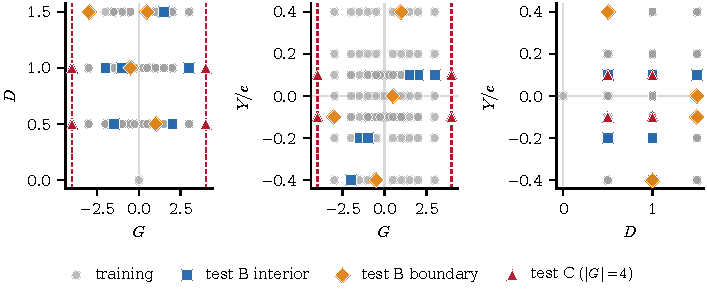
\includegraphics[width=\linewidth]{sections/figures/results/fig_paramspace_v3.pdf}
  \caption{\rb{K}{S2-C3}{Shows the sampling and the symmetric boundary, and names the $Y$ under-sampling that \S5.4 lists as a limitation.}Parameter-space sampling of the $\NCases$ cases in the $(G, D, Y)$ gust
  envelope, shown as three two-dimensional projections and coloured by split:
  training ($\NTrainEnc$ encounters), the stratified in-distribution test set
  ($\NTestBEnc$ encounters from $\NTestBCases$ cases, split into in-distribution
  and edge-of-training tiers), and the $|G| = 4$ extrapolation set
  ($\NTestCEnc$ encounters from $\NTestCCases$ cases). The dashed lines mark the
  $|G| = 4$ extrapolation boundary, now sampled at both signs of the gust so that
  the boundary set is symmetric rather than one-sided. Training mass concentrates
  near $Y/c = 0$, which is why the wall-normal offset is the least well resolved
  parameter (\S\ref{sec:res_latent_physics}).\re}
  \label{fig:paramspace}
\end{figure}


\section{Predictive latent representation and evaluation protocol}
\label{sec:methods}
% Predictive latent representation and evaluation protocol. Former Section 3
% (Methods), compressed and de-diaried. JFM structure pass: five subsections
% reduced to three (model+objective+conditioning; closure protocol;
% diagnostics/controls/uncertainty), the two run-in \emph headings of the old
% diagnostics subsection rewritten as prose, and the two method schematics
% combined into one figure (architecture + evaluation protocol) with the
% predictive-vs-reconstructive contrast moved to Appendix~\ref{app:reg}.

\subsection{Model, training objective, and conditioning split}
\label{sec:methods_arch}
\label{sec:methods_loss}

The predictive encoder $E_\theta$ maps the mid-plane vorticity field
$\omegaz(192,96)$ to a latent $\zvec \in \mathbb{R}^d$ at $d \in \{16, 32, 64\}$. It
is a hybrid network: three convolutional downsampling stages produce a
$24 \times 12 \times 256$ feature map, a six-layer vision transformer processes
the resulting tokens, and the class-token output is projected to $\zvec$ through
a single linear layer with a batch-normalisation boundary, which the
characteristic-function regulariser below requires. The encoder is
\emph{unconditional} by design: it sees only the flow field, not the gust
parameters $\cvec = (G,D,Y)$. This is the property that lets the latent itself
serve as the observable a controller would have access to, since at deployment
the gust parameters are not known a priori (\S\ref{sec:discussion}). The
conditional predictor, by contrast, still requires $\cvec$, either estimated
from the wall or marginalised over, so an observable latent is a necessary but
not a sufficient condition for a deployable forward model.

The predictor $P_\phi$ advances the latent in time. It is a six-layer
autoregressive transformer with rotary positional embeddings and a causal mask,
conditioned on $\cvec$ through adaptive layer-norm modulation at every block;
its internal structure is given in Appendix~\ref{app:reg}. The predictor is the only stage
that sees $\cvec$. Figure~\ref{fig:method}(a) shows the encoder and
predictor, and panel~(b) sets out the matched-predictor evaluation protocol used
throughout; the contrast between the predictive training signal and the
reconstructive one, in which the reconstructive autoencoder passes the field at
time $t$ through an encoder and a decoder and incurs a field-space error whereas
the predictive model encodes the fields at $t$ and $t+\Delta t$ with shared
weights and incurs a latent-space error between the predicted and observed target
embeddings, with no field-space loss, is drawn in Appendix~\ref{app:reg}
(figure~\ref{fig:predictive_vs_reconstructive}).
Table~\ref{tab:architecture} summarises the two networks.

\begin{table}
  \centering
  \caption{Encoder and predictor configuration. The encoder is unconditional;
  the gust parameters $\cvec = (G,D,Y)$ enter only
  the predictor, through identity-initialised adaptive layer normalisation
  (AdaLN-Zero). Parameter counts are for the $d = 64$ configuration; two small
  auxiliary heads read observables off the encoder output during training (a lift
  head, $4\times10^{3}$ parameters, and an $80$-dimensional wake-spectrum head,
  $3.5\times10^{4}$ parameters; \S\ref{sec:methods_loss}).}
  \label{tab:architecture}
  \small
  \fittab{\begin{tabular}{l l l}
    \toprule
     & Encoder $E_\theta$ & Predictor $P_\phi$ \\
    \midrule
    role            & field $\to$ latent (unconditional) & latent dynamics (conditioned) \\
    input           & $\omegaz \in \mathbb{R}^{192 \times 96}$ & latent sequence $\zvec_{1:t}$ \\
    backbone        & 3 conv.\ stages $+$ 6-layer ViT & 6-layer autoregressive transformer \\
    width / heads   & $256$ / $8$ & $384$ / $16$ \\
    tokens / context & $24 \times 12 = 288$ spatial & $\le 32$ temporal (causal) \\
    conditioning    & none & AdaLN-Zero on $\cvec = (G,D,Y)$, rotary time \\
    latent read-out & class token $\to$ linear $\to$ BatchNorm & next-step latent \\
    parameters      & $6.7$M & $16.2$M \\
    \bottomrule
  \end{tabular}}
\end{table}

The predictive encoder and predictor are trained jointly on a one-step
latent-prediction term, a scheduled-sampling rollout term that exposes the
predictor to its own errors, and an anti-collapse regulariser that prevents the
encoder from collapsing to a constant. We use the characteristic-function
regulariser of \citet{lejepa,lewm}, which matches the latent distribution to an
isotropic Gaussian through a small number of random projections, with an
automatic fall-back to a variance-covariance objective \citep{vicreg} should the
participation ratio of the latent indicate collapse. Its configuration is given
in Appendix~\ref{app:reg}.

Two auxiliary heads read aerodynamic observables off the encoder output during
training: a lift head that maps $\zvec_t$ to $C_L(t)$, and a wake head that maps
$\zvec_t$ to an $80$-dimensional signed wake spectrum, both trained with small
weights jointly with the representation and neither part of the latent-prediction
loss. These heads are adopted from the observable-augmentation
lineage \citep{fukami2023,fukami2025}. They are also, however, the reason the
present predictive encoder is not a clean isolation of the training objective:
the reconstructive baseline below carries a lift head but not a wake head, and
the two encoders differ in architecture as well. We are explicit about this
throughout. The headline comparison is therefore between encoder
\emph{families} as configured, and the controls of \S\ref{sec:res_controls}
are designed to separate the objective from the architecture and the wake
supervision.

\begin{figure}
  \centering
  \begin{subfigure}{\linewidth}
    \centering
    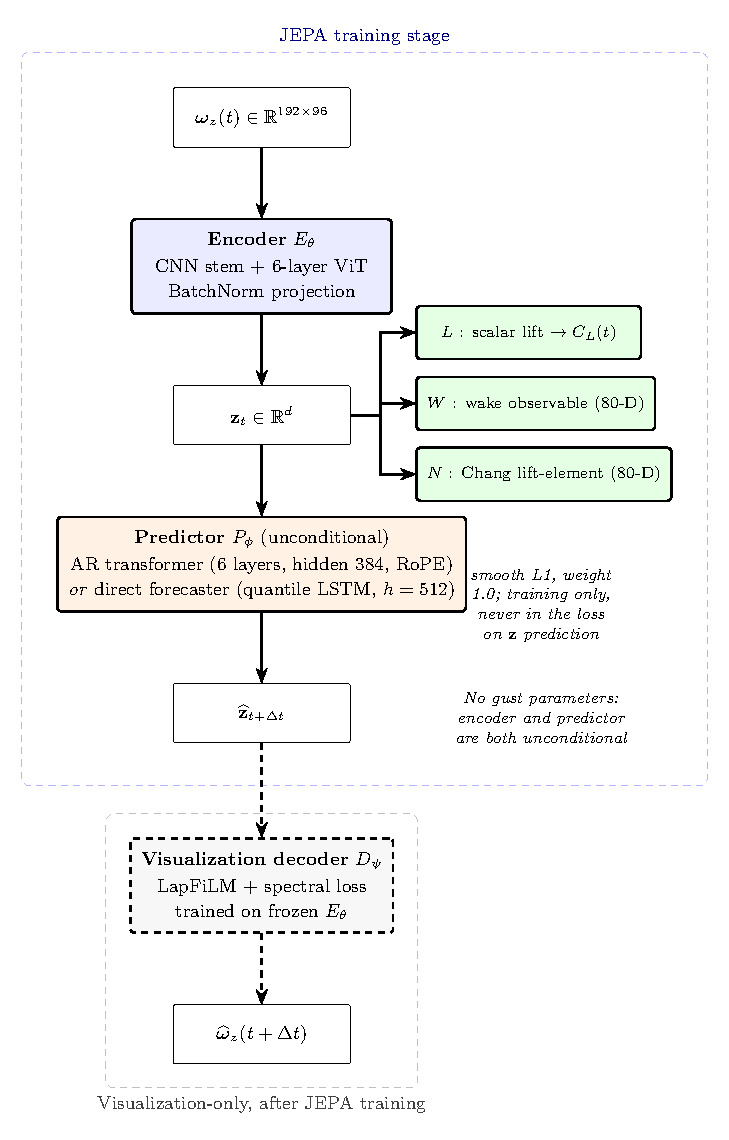
\includegraphics[width=0.52\linewidth]{sections/figures/tikz/fig1_jepa_architecture.pdf}
    \caption{}
    \label{fig:method_arch}
  \end{subfigure}
  \\[1.5ex]
  \begin{subfigure}{\linewidth}
    \centering
    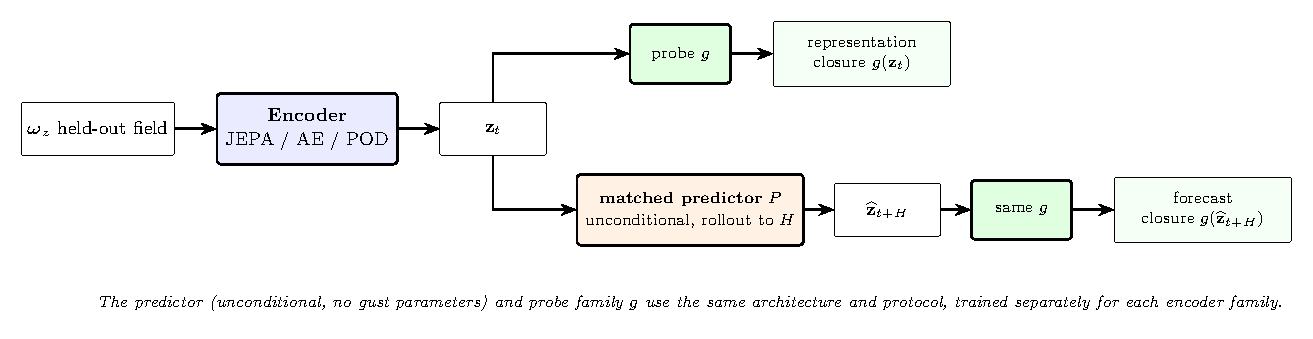
\includegraphics[width=0.98\linewidth]{sections/figures/tikz/fig_eval_protocol.pdf}
    \caption{}
    \label{fig:method_eval}
  \end{subfigure}
  \caption{The predictive model and how it is evaluated. (a) The encoder is
  unconditional and maps the mid-plane vorticity field to a latent $\zvec_t$,
  while the autoregressive predictor advances the latent given the gust
  conditioning $\cvec = (G,D,Y)$, which enters the predictor alone. The two
  auxiliary observable heads (lift and wake) read $\zvec_t$ during JEPA training
  with small weights and are not part of the latent-prediction loss; they are
  omitted from the schematic for clarity. The visualisation decoder is trained
  only after the encoder is frozen and is used solely for the diagnostic decodes
  of \S\ref{sec:res_physical}, never in the predictive loss. (b) Evaluation
  applies the same predictor architecture, conditioning, and probe family $g$, each
  trained or fitted separately per encoder family: a probe on the simulation-encoded
  latent measures representation
  closure, and the same probe on the rolled-out latent $\widehat{\zvec}_{t+H}$
  measures forecast closure.}
  \label{fig:method}
\end{figure}

\subsection{Matched-predictor closure protocol}
\label{sec:methods_protocol}
\label{sec:methods_closure}

The comparison rests on a single principle: every baseline is the same
three-stage pipeline, and only the encoder differs. Each encoder produces a
latent trajectory $\zvec_{1:T}$ from the vorticity fields; an identical
autoregressive transformer predictor rolls it forward one step at a time given
$\cvec$; and an identical probe family maps the predicted latent to a physical
observable for evaluation (figure~\ref{fig:method}(b)). The predictor
architecture, its training recipe, the parametric conditioning, and the probe
family are held fixed across the three encoder families. The latent dimension
is matched within each family: JEPA at $d \in \{16, 32, 64\}$, the reconstructive
autoencoder at $d \in \{3, 32, 64\}$ to include both the published $d = 3$
recipe and matched-capacity variants, and POD at $d \in \{16, 32, 64\}$. The
predictive family is additionally swept to $d \in \{4, 8\}$ and ablated without its
predictor conditioning in \S\ref{sec:res_controls}. This
isolation is the only fair way to attribute forecast quality to the
representation rather than to incidental differences in the predictor or its
training. The reconstructive autoencoder uses its best-documented configuration,
with ReLU activations, group normalisation, and a future-lift head at horizons
$\{8, 16, 24\}$, rather than the strict published variant (tanh, no normalisation,
a current-lift head), which we found gives a worse parametric probe; the
comparison is therefore against a tuned baseline, not a hobbled one.

The figure of merit is forward physical closure, the empirical test of the
geometric criterion set out in the introduction: a latent whose metric stays
aligned with the transport geometry under the predictor keeps each observable
recoverable along the rollout, while one that drifts off the manifold loses it. Given a ground-truth
$\cvec$ and an initial latent, the predictor is rolled recursively to $H = 16$, and
at each step the probe maps the predicted latent to each observable. A small
closure error means the encoder produces a latent whose dynamics, propagated by
the predictor, retain the information the probe needs to recover the
physical quantity; a large error means either that the encoder discarded that
information or that the predictor lost it during rollout, a distinction the
drift diagnostic below resolves. We report closure on the held-out test\_b and
test\_c encounters as the mean absolute error against the simulation, with
bootstrap $95\%$ confidence intervals over encounters and the coefficient of
determination $R^2$.
%
% HONESTY NOTE: the original draft headed the results with a *training-set* R^2
% (mean 0.835). That number is retained only as a training-fit reference
% (table~\ref{tab:b1_closure_train_r2}); the headline is the held-out error.
% test_b / test_c R^2 computed from the same rollout predictions used for the
% held-out MAE and reported in table~\ref{tab:closure} panel (b) (forecast) and
% panel (a) (representational closure).
The held-out forecast $R^2$ (Markov rollout at $H = 16$) is reported in
table~\ref{tab:closure}(b), and the representational closure (probe on the
simulation-encoded latent) in table~\ref{tab:closure}(a).

\subsection{Diagnostics, controls, and uncertainty}
\label{sec:methods_diag}

Two diagnostics turn the closure number into a mechanism. The first is the
latent drift, which addresses the fact that a predictor with low one-step error
need not produce a useful long rollout, because each prediction is fed back as
the next input and small geometric errors accumulate. We quantify how far a
rollout has left the training manifold by the Mahalanobis distance of the
rolled-out latent at horizon $H$, measured against the distribution of
simulation-encoded latents for the same encoder, normalised by the Mahalanobis
distance of the simulation-encoded latent itself. A ratio near one means the
rollout stays within the natural spread of the training latents; a large ratio
means it has gone out of distribution, so that the probe is then queried outside
its support.

The second diagnostic is a conditioning-only floor. Because the predictor is
conditioned on $\cvec = (G,D,Y)$, a natural concern is that the forecast quality
is carried by the conditioning rather than by the latent. We bound this with a
kernel-ridge regressor that maps $\cvec$ directly to each observable at the
forecast horizon $H = 16$, with no latent input, fit on training and evaluated on
the held-out splits, so that it is frame-matched to the closure it is compared
against. This is the floor any learned encoder must clear at that horizon to
demonstrate that its latent contributes beyond what is already implicit in the
parameters. At the impact frame the same parameter floor is high, because the
just-released gust nearly determines the instantaneous state; the predictive
latent must instead close the gap that opens as the wake evolves
(\S\ref{sec:res_closure}).

Because the predictive encoder differs from the reconstructive baseline in
objective, architecture, and auxiliary supervision at once, the comparison is
accompanied by controls that vary one factor at a time: a crossing of objective
with architecture at matched auxiliary heads, an ablation of each auxiliary head,
and an ablation of the predictor conditioning (\S\ref{sec:res_controls}). Every
held-out $R^2$ and mean absolute error reported below carries three independent
uncertainty signals, following the reporting protocol fixed with the data split:
a $2000$-resample bootstrap over the held-out encounters, the standard deviation
across three encoder retrains from independent seeds, and a five-fold
cross-validation over cases on the probe read-out. Their full specification is in
Appendix~\ref{app:reg}.


\section{Results}
\label{sec:results}
% Results, restructured by physical question. Five subsections (JFM structure
% pass): (1) forward closure and conditioning floor; (2) objective/architecture/
% auxiliary-head controls (kept ahead of the mechanism, because architecture and
% wake supervision are confounds); (3) why the rollout works, folding horizon
% dependence into the drift/topology/transport mechanism; (4) where closure
% succeeds and fails in physical space, folding parameter/phase dependence into
% the decoded-field interpretation; (5) wall-pressure observability. The seven
% former run-in \paragraph labels are rewritten as prose. Every result is
% populated.

% Tables for the Results section. Only the two tables discussed at the very top
% of Section 4 (the families overview and the headline closure table) live here
% and are \input at the start of the section. The later tables (conditioning
% floor, latent drift, 2x2 controls) are placed inline next to their first
% reference, further down the section, so floats land near their discussion.

% ---------------------------------------------------------------------------
% TABLE: model families and objectives (new; standard JFM summary table).
% ---------------------------------------------------------------------------
\begin{table}[t]
  \centering
  \caption{Encoder families compared under the matched-predictor protocol of
  \S\ref{sec:methods_protocol}. All three share one autoregressive transformer
  predictor, training recipe, conditioning on $\cvec=(G,D,Y)$, and probe family;
  only the encoder differs. ``Aux.\ heads'' lists the observable supervision
  attached to the encoder. The architecture and auxiliary-head columns differ
  across families, which is why the headline result is attributed to the
  predictive \emph{family} and isolated only by the controls of
  \S\ref{sec:res_controls}.}
  \label{tab:families}
  \small
  \begin{tabular}{l l l l l}
    \toprule
    Family & Objective & Encoder & Latent dim.\ $d$ & Aux.\ heads \\
    \midrule
    JEPA (this work) & predictive (latent) & CNN $+$ ViT & $16,\,32,\,64$ & lift $+$ wake \\
    Reconstructive AE & reconstructive (field) & CNN & $3,\,16,\,32,\,64$ & lift \\
    POD & linear projection & --- & $16,\,32,\,64$ & --- \\
    \bottomrule
  \end{tabular}
\end{table}

% ---------------------------------------------------------------------------
% TABLE: held-out closure (test_b MAE). THIS IS THE HEADLINE TABLE.
% ---------------------------------------------------------------------------
\begin{table}[t]
  \centering
  \caption{Held-out closure across encoder families at $H = 16$ on the $n = 42$
  test\_b encounters, in two modes. \emph{(a)} Representational closure: the mean
  absolute error when each family's per-frame probe is applied to the
  simulation-encoded latent (the latent encoded directly from the held-out field),
  smaller is better. \emph{(b)} Forecast closure: the coefficient of determination
  $R^2$ of the Markov rollout from the impact frame against the simulation
  observable, larger is better (the variance baseline is the held-out split mean,
  so $R^2 < 0$ is worse than predicting that mean). Best per column in bold; the
  forecast panel gives the row mean at right. The wake-enstrophy and circulation
  columns are in native units, the force coefficients dimensionless. This held-out
  forecast $R^2$, not the training-set fit of
  Table~\ref{tab:b1_closure_train_r2}, is the reported closure quality. The
  predictive latent leads in both modes: its representational wake-enstrophy error
  is $2.4$ to $3.0$ times lower than the reconstructive and linear families, and
  its forecast wake-enstrophy $R^2$ is the only one above the predict-the-mean
  floor; the paired per-encounter test is in Table~\ref{tab:paired_closure} and
  full probe values with bootstrap CIs are in Appendix~\ref{app:reg}.}
  \label{tab:closure}
  \small
  \begin{tabular}{l c c c c c c c}
    \multicolumn{8}{c}{\textit{(a) Representational closure: mean absolute error}}\\
    \toprule
    Baseline & $d$ & $C_L$ & $C_D$ & $I_y$ & wake-enst.\ & circ.\ pos.\ & circ.\ neg.\ \\
    \midrule
    JEPA   & 64 & \textbf{0.624} & 0.301 & \textbf{1.901} & \textbf{29.83} & \textbf{0.801} & \textbf{0.715} \\
    JEPA   & 32 & 0.675 & \textbf{0.246} & 2.976 & 37.99 & 1.084 & 1.061 \\
    JEPA   & 16 & 0.627 & 0.267 & 2.883 & 50.09 & 0.939 & 1.322 \\
    \midrule
    Fukami & 3  & 1.074 & 0.384 & 2.327 & 51.70 & 1.110 & 1.886 \\
    Fukami & 32 & 1.038 & 0.368 & 2.195 & 63.94 & 0.946 & 1.789 \\
    Fukami & 64 & 0.989 & 0.340 & 2.421 & 72.90 & 1.057 & 1.904 \\
    Fukami & 16 & 1.133 & 0.421 & 2.424 & 77.26 & 1.158 & 1.837 \\
    \midrule
    POD    & 16 & 1.168 & 0.317 & 2.235 & 89.14 & 1.645 & 1.681 \\
    POD    & 32 & 0.937 & 0.269 & 2.608 & 81.82 & 1.650 & 1.617 \\
    POD    & 64 & 0.872 & 0.291 & 2.245 & 89.31 & 1.660 & 1.800 \\
    \bottomrule
  \end{tabular}

  \vspace{6pt}

  \begin{tabular}{l c c c c c c c c}
    \multicolumn{9}{c}{\textit{(b) Forecast closure: coefficient of determination $R^2$}}\\
    \toprule
    Baseline & $d$ & $C_L$ & $C_D$ & $I_y$ & wake-enst.\ & circ.\ pos.\ & circ.\ neg.\ & mean \\
    \midrule
    JEPA   & 64 & 0.723 & 0.634 & 0.056 & \textbf{0.449} & 0.201 & \textbf{0.607} & \textbf{0.445} \\
    JEPA   & 32 & \textbf{0.751} & \textbf{0.648} & -0.082 & 0.214 & 0.087 & 0.552 & 0.362 \\
    JEPA   & 16 & 0.642 & 0.465 & 0.002 & 0.265 & 0.250 & 0.557 & 0.363 \\
    \midrule
    Fukami & 3  & 0.632 & 0.226 & 0.115 & -0.082 & 0.258 & -0.048 & 0.184 \\
    Fukami & 32 & 0.641 & 0.239 & \textbf{0.205} & 0.007 & \textbf{0.420} & 0.161 & 0.279 \\
    Fukami & 64 & 0.729 & 0.406 & 0.043 & -0.478 & 0.182 & 0.003 & 0.147 \\
    Fukami & 16 & 0.565 & 0.125 & -0.216 & -0.395 & 0.237 & 0.225 & 0.090 \\
    \midrule
    POD    & 16 & 0.499 & 0.364 & -0.515 & -0.129 & -0.230 & 0.340 & 0.055 \\
    POD    & 32 & 0.714 & 0.558 & -0.256 & 0.042 & -0.066 & 0.394 & 0.231 \\
    POD    & 64 & 0.683 & 0.539 & -0.813 & -0.089 & 0.057 & 0.507 & 0.147 \\
    \bottomrule
  \end{tabular}
\end{table}


\subsection{Representational wake closure and the parameter-only floor}
\label{sec:res_closure}

Table~\ref{tab:families} summarises the three encoder families and the protocol.
We distinguish two questions. Does the latent, encoded directly from a held-out
field, render each observable readable by a fixed linear probe (representation
quality, the headline, table~\ref{tab:closure}(a))? And does the predictor, rolled
out from the impact frame, track it (forecast quality, reported as secondary,
table~\ref{tab:closure}(b))? The first isolates the encoder; the second tests the
encoder and the learned dynamics together. The result is established at the
representation level, where the wake is the discriminator, and the rollout is shown
as consistent confirmation rather than the load-bearing test.

The wake is where the families separate. Probed directly from the held-out field
sixteen frames after impact, the predictive latent renders the wake enstrophy
linearly readable at $R^2 = \NumReprWakeJepaTf$ (figure~\ref{fig:fig4_closure}),
while the reconstructive autoencoder and the linear basis are at
$\NumReprWakeFukami$ and $\NumReprWakePod$, both below the predict-the-mean floor.
A nonlinear (kernel-ridge) probe narrows this gap, recovering part of the wake from
the matched-head reconstructive control (\S\ref{sec:res_controls}), so the claim is
that the predictive objective renders the wake \emph{linearly decodable}, not that
the reconstructive encoding discards it irrecoverably. The forces and the
circulations are read off the same latent cleanly, with $C_L$ at
$R^2 = \NumCloReprCLJepaTf$, the negative and positive circulations at
$\NumCloReprCircNegJepaTf$ and $\NumCloReprCircPosJepaTf$, and the drag at
$\NumCloReprCDJepaTf$; the mean over the six observables is
$\NumCloReprMeanSixJepaTf$. The one weak observable is the wall-normal impulse $I_y$
($R^2 = \NumCloReprIyJepaTf$), a mid-plane vorticity diagnostic that even the
energy-optimal linear basis captures only modestly (\S\ref{sec:flow_observables}),
so its weakness is a property of the observable rather than of the predictive
latent. The same ordering holds on the training, validation, and extrapolation
(test\_c) splits reported below.

\begin{figure}
  \centering
  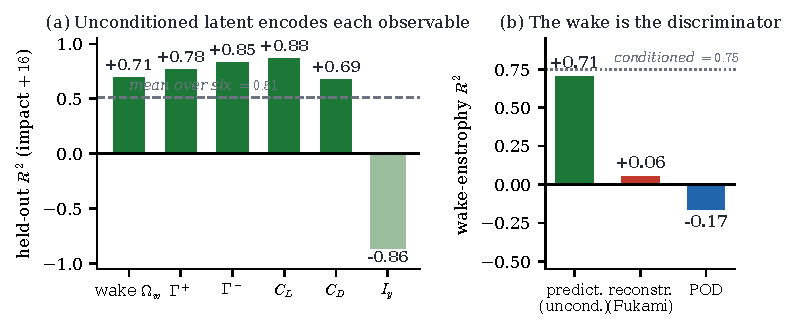
\includegraphics[width=\linewidth]{sections/figures/results/fig4_closure.pdf}
  \caption{Representational closure of the predictive latent at $H = 16$ after gust
  impact, the headline result. (a) Held-out $R^2$ of a fixed linear probe applied to
  the simulation-encoded latent (no rollout) for each of the six observables, on the
  in-distribution test set (test\_b, $n = 42$); the dashed line marks the mean over
  the six and the one weak observable, the mid-plane impulse $I_y$, is shaded light.
  (b) The wake-enstrophy $R^2$ across families: the predictive latent
  ($\NumReprWakeJepaTf$) against the reconstructive autoencoder
  ($\NumReprWakeFukami$) and the linear basis ($\NumReprWakePod$), each at $d = 64$.
  The wake is the discriminator, and only the predictive latent renders it linearly
  readable.}
  \label{fig:fig4_closure}
\end{figure}

The rollout points the same way and is read as confirmatory, not as the headline
(table~\ref{tab:closure}(b) and figure~\ref{fig:traces}). A matched transformer
predictor is trained on each family's latents under one protocol, and rolled out
from the full pre-impact context; probing the wake enstrophy at $H = 16$, the
forecast $R^2$ is $\NumCloFcstWakeJepaTf$ for the predictive latent, ahead of
$\NumCloFcstWakeFukami$ for the reconstructive autoencoder and
$\NumCloFcstWakePod$ for the linear basis. The forecast ordering is the same as the
representational one but compressed, which is why we lead with the representation:
the families separate most cleanly at the encoder, and the rollout confirms rather
than carries the result. The forecast advantage is not statistically separable
under case-level clustering (\S\ref{sec:res_drift} and
table~\ref{tab:paired_closure}), so we present it as consistent tracking, not as a
forecast claim. On the extrapolation set (test\_c, $G = +4$) the predictive
wake-enstrophy forecast stays the strongest of the three while the integrated
forces collapse, consistent with the three-dimensional observability boundary of
\S\ref{sec:flow_physics}.

\begin{figure}
  \centering
  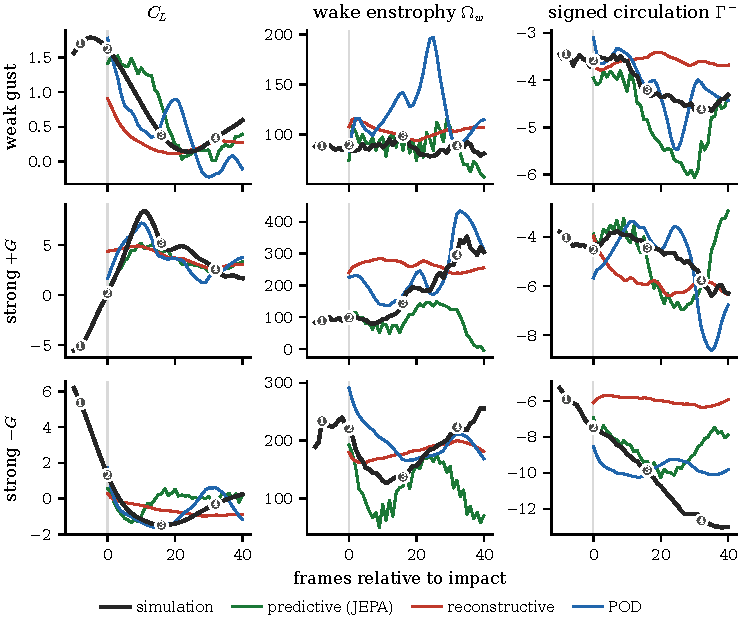
\includegraphics[width=\linewidth]{sections/figures/results/figA_traces.pdf}
  \caption{The predictive rollout tracks the encounter, shown qualitatively.
  Predicted observables through representative held-out encounters (rows), for the
  lift coefficient, the wake enstrophy, and the negative circulation (columns). The
  simulation is the bold reference; the rollout of the predictor, started from the
  pre-impact context, is the coloured line, and the dashed line is the
  reconstruction from the encoded latent. The rollout tracks the
  wake observables through the leading-edge-vortex peak and into recovery before
  drifting gently at long times. We report this as qualitative tracking, not as a
  closure $R^2$. Numbered glyphs mark the four encounter stages used throughout:
  baseline, impact, peak load, and recovery.}
  \label{fig:traces}
\end{figure}

The representational wake separation is the statistically robust core of the
result. A per-encounter paired test (table~\ref{tab:paired_closure}), which cancels
the encounter-to-encounter difficulty of the held-out set that every model shares,
shows the predictive latent carrying the smaller wake-enstrophy error under direct
encoding by a paired margin of $\NumPairedWakeRepr$ (case-clustered $95\%$ CI
$[\NumPairedWakeReprlo, \NumPairedWakeReprhi]$, excluding zero). We report the
multiplicity correction at two levels and state honestly where the advantage
stops: the representational wake-enstrophy advantage survives the pre-registered
encounter-level family correction (one of $\NumHolmSurvivors$ of twelve paired
tests that survive Holm, together with the lift and the negative circulation),
but it does not survive the stricter case-level correction, where the smaller
number of held-out cases widens the interval. The forecast advantage points the
same way but survives neither. All six observables are reported in both modes, not
a selected subset, and the ordering is not uniform: the predictive latent leads on
the spatially distributed wake observables (enstrophy and negative circulation),
which is precisely the paper's claim. This separation is confirmed by the
mechanistic evidence of \S\ref{sec:res_drift} (the drift departure spectrum and the
no-gust limit-cycle topology), where the predictive and reconstructive families
separate consistently.

\begin{table}
  \centering
  \caption{Parametric (model-free) floor at $H = 16$ after impact. A
  cross-validated ridge regressor maps the gust parameters $\cvec = (G,D,Y)$
  directly to each observable, with no latent input, fit on the training cases and
  read out on the in-distribution test split under the closure protocol
  ($R^2 = 1 - \mathrm{SSE}/\mathrm{SST}$ about the held-out mean). This is the
  model-free baseline: the predictive latent beating it (last column, the
  representational closure of table~\ref{tab:closure}(a)) shows the representation
  carries flow state the parameters alone do not supply. On wake enstrophy the
  floor is negative ($R^2 = \NumFloorWake$): the gust parameters alone do worse than
  the held-out mean sixteen frames after impact, because the wake is then governed
  by the unfolding dynamics rather than by the release condition, whereas the
  predictive latent reads it at $\NumReprWakeJepaTf$. On the forces, which track the
  gust forcing more directly, the floor is high.
  }
  \label{tab:parametric_floor}
  \small
  \fittab{\begin{tabular}{l c c}
    \toprule
    Observable & parametric floor (test\_b $R^2$) & predictive repr.\ (test\_b $R^2$) \\
    \midrule
    $C_L$          & \NumFloorCL      & \NumCloReprCLJepaTf \\
    $C_D$          & \NumFloorCD      & \NumCloReprCDJepaTf \\
    $I_y$          & \NumFloorIy      & \NumCloReprIyJepaTf \\
    wake-enstrophy & \NumFloorWake    & \NumReprWakeJepaTf \\
    circ.\ pos.\   & \NumFloorCircPos & \NumCloReprCircPosJepaTf \\
    circ.\ neg.\   & \NumFloorCircNeg & \NumCloReprCircNegJepaTf \\
    \bottomrule
  \end{tabular}}
\end{table}

The parametric floor (table~\ref{tab:parametric_floor}) confirms that the wake
closure is not something the gust parameters supply on their own. Mapping
$\cvec = (G,D,Y)$ to each observable at $H = 16$ with cross-validated regressors,
the floor on wake enstrophy is negative ($R^2 = \NumFloorWake$ for the linear
regressor, $\NumParamFloorWakeKrr$ for the nonlinear one): the parameters alone do
worse than predicting the held-out mean, while the predictive latent reads the wake
at $\NumReprWakeJepaTf$, clearing the floor by roughly $0.9$. The floor is by
construction strong on the observables that track the gust forcing directly, the
lift ($\NumFloorCL$) and the negative circulation ($\NumFloorCircNeg$): the
predictive advantage is specific to the spatially distributed wake, not uniform
across observables, and this is the paper's central distinction between the
integrated forces, which the release condition largely fixes, and the wake, which
it does not. The wake claim therefore rests on the representational closure
(table~\ref{tab:closure}(a)), the per-encounter paired test
(table~\ref{tab:paired_closure}), and the drift mechanism (\S\ref{sec:res_drift}),
with the parametric floor establishing that the gust parameters do not supply the
wake state the latent encodes.

\subsection{Objective, architecture, and auxiliary-head controls}
\label{sec:res_controls}

The representational result of \S\ref{sec:res_closure} is established, but the
predictive latent \emph{family} as configured renders the wake readable for reasons
we have not yet separated: the predictive encoder differs from the reconstructive
baseline not only in its training objective but also in its CNN$+$ViT architecture
and its $80$-dimensional wake supervision. Because the architecture and the wake
supervision are confounds, we isolate the cause here, before turning to why the
rollout stays on the manifold (\S\ref{sec:res_drift}). The controls in
table~\ref{tab:controls_2x2} are the decisive crossing, run directly on the same
models the paper reports and scored at the representational endpoint: a
$2 \times 2$ crossing of objective \{predictive, reconstructive\} with architecture
\{CNN, CNN$+$ViT\} at matched $d = 64$, with the auxiliary heads matched across all
four cells, together with a predictive variant from which the wake head is removed.
The decisive question is whether the predictive objective renders the wake readable
more than the reconstructive one once the architecture and the wake supervision are
held in common.

\begin{table}
  \centering
  \caption{Objective $\times$ architecture controls (decisive experiment), scored
  at the representational endpoint on the in-distribution test split. Held-out
  representational wake-enstrophy $R^2$ at $H = 16$ (test\_b, fixed linear probe on
  the simulation-encoded latent, seed mean) for the four cells crossing
  \{predictive, reconstructive\} with \{CNN, CNN$+$ViT\} at $d = 64$, with the
  auxiliary heads (the instantaneous lift plus the $80$-dimensional wake head)
  matched across all four cells, plus a predictive variant with the wake head
  removed. Predictive renders the wake readable at both architectures, while both
  reconstructive cells stay low; removing the wake head from the predictive model
  collapses wake readability to the floor, so the wake supervision is also
  necessary. The CNN and CNN$+$ViT predictive columns do not separate, so the ViT
  is not the driver.}
  \label{tab:controls_2x2}
  \small
  \fittab{\begin{tabular}{l l l c}
    \toprule
    Objective & Encoder & Aux.\ heads & repr.\ wake-enst.\ $R^2$ \\
    \midrule
    predictive     & CNN$+$ViT & lift $+$ wake & $\mathbf{\NumReprWakeJepaTf}$ \\
    predictive     & CNN       & lift $+$ wake & $\NumReprWakeCtrlPredCnn$ \\
    reconstructive & CNN$+$ViT & lift $+$ wake & $\NumReprWakeCtrlReconCnnVit$ \\
    reconstructive & CNN       & lift $+$ wake & $\NumReprWakeCtrlReconCnn$ \\
    \midrule
    predictive     & CNN$+$ViT & lift only     & $\NumReprWakeCtrlPredVitNowake$ \\
    \bottomrule
  \end{tabular}}
\end{table}

The controls (table~\ref{tab:controls_2x2}) give a two-part answer, and we state
both. First, the predictive objective renders the wake readable at \emph{both}
architectures with the auxiliary heads matched: the representational
wake-enstrophy $R^2$ is $\NumReprWakeJepaTf$ for the predictive CNN$+$ViT and
$\NumReprWakeCtrlPredCnn$ for the predictive CNN, while both reconstructive cells
stay low ($\NumReprWakeCtrlReconCnnVit$ at CNN$+$ViT, $\NumReprWakeCtrlReconCnn$ at
CNN). The objective, not the architecture, carries the advantage: the two
predictive columns do not separate, so the ViT is not the driver. Second, and
equally important, the wake-observable supervision is necessary: the predictive
model with the wake head removed collapses to a representational wake $R^2$ of
$\NumReprWakeCtrlPredVitNowake$, at the floor and below every other predictive
cell. The result therefore requires the predictive objective \emph{and} the wake
supervision together; it is not a property of the objective in isolation, nor of
the architecture, nor of the wake head attached to an arbitrary objective (the
reconstructive cells carry the same wake head and do not reach the predictive
readability). We claim, accordingly, that the predictive objective renders the
wake linearly readable over the reconstructive objective at matched architecture
and matched supervision, with the auxiliary wake head a necessary component of the
configuration that achieves it.

The latent dimension is the remaining control. The representational wake closure
holds on a plateau from $d = 64$ down to $d = 16$ ($R^2 = \NumCloReprWakeJepaTfDSixtyfour$,
$\NumCloReprWakeJepaTfDThirtytwo$, and $\NumCloReprWakeJepaTfDSixteen$ at $d = 64$, $32$,
and $16$) and falls off below, so the reported $d = 64$ sits on the plateau and the
wake is not recoverable at the smallest dimensions on this dataset. The latent code
is correspondingly distributed rather than concentrated in a few coordinates, which
\S\ref{sec:res_code} makes quantitative.

\subsection{Why the latent stays on the manifold: drift, topology, and transport}
\label{sec:res_horizon}
\label{sec:res_drift}

The controls attribute the wake advantage to the predictive objective trained
with wake supervision, and the representation is where that advantage is
established. A separate question is whether the latent is usable under rollout,
since a planner queries a forward model at the states its own rollout reaches. The
answer is geometric: the unconditioned predictive latent stays on its encoded
manifold while the reconstructive one drifts off, which we establish first as a
horizon-resolved rollout drift and then with three coordinate-free diagnostics of
the rollout itself.

The unconditioned rollout drifts gracefully. Rolling the unconditioned predictor
forward and measuring the relative deviation of the rolled latent from the latent
encoded directly from the simulation, as a fraction of the encoded-latent scale, the
drift grows gradually with horizon and stays bounded
(figure~\ref{fig:drift_uncond}), and it tracks the conditioned model closely, so
removing the gust parameters does not destabilise the rollout. This is the property a
forward model needs and it is why the qualitative rollout of figure~\ref{fig:traces}
tracks the encounter through impact before drifting only at long times. We do not
attach a forecast $R^2$-versus-horizon headline to this rollout; the representational
closure of \S\ref{sec:res_closure} carries the result, and the rollout is shown to be
on-manifold and usable.

\begin{figure}
  \centering
  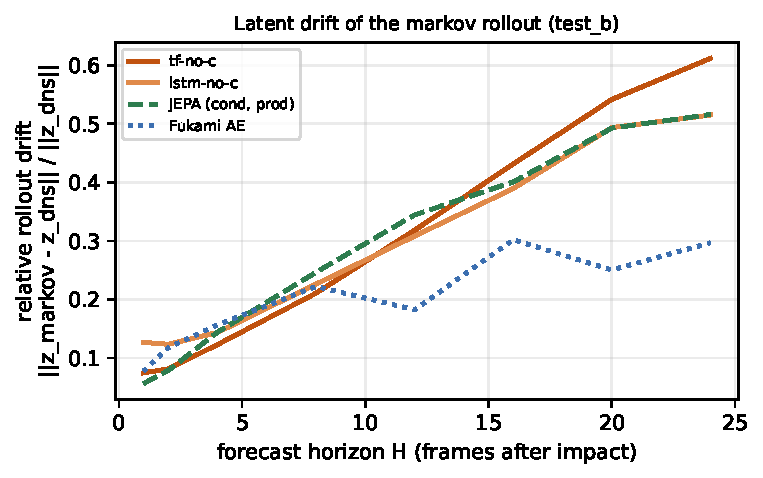
\includegraphics[width=0.7\linewidth]{sections/figures/results/fig_horizon_sweep.pdf}
  \caption{Relative drift of the unconditioned rollout on test\_b versus forecast
  horizon $H$, measured as the deviation of the rolled latent from the
  simulation-encoded latent normalised by the encoded-latent scale,
  $\lVert \widehat{\zvec}_{\text{rollout}} - \zvec_{\text{DNS}}\rVert /
  \lVert \zvec_{\text{DNS}}\rVert$. The unconditioned transformer predictor (tf-no-c)
  and a recurrent unconditioned variant (lstm-no-c) drift gradually and track the
  conditioned production model closely, so dropping the gust parameters does not
  destabilise the rollout. This is a deviation diagnostic of the unconditioned model,
  not a forecast-$R^2$ headline; the family-separating drift is the Mahalanobis
  manifold-departure of table~\ref{tab:latent_drift}.}
  \label{fig:drift_uncond}
\end{figure}

The drift behaviour points to a geometric cause, which the rest of this
subsection establishes three ways that do not
depend on the latent coordinates: a distance that shows whether the rollout leaves
the training manifold, a topology that shows whether the encounter stays a single
cycle, and an optimal-transport metric that shows whether latent distance tracks the
physical rearrangement of the flow. Together they test the one property a predictive
objective confers and a reconstruction objective does not, that the latent metric
stays aligned with the transport geometry under the predictor step, so the rollout
remains close to the encoded manifold.

\begin{table}
  \centering
  \caption{Latent-drift diagnostic on test\_b at $H = 16$. The Mahalanobis
  distance of the rolled-out latent is reported alongside that of the
  simulation-encoded latent in the same reference distribution; their ratio
  $r = d_{\text{Mahal, Markov}} / d_{\text{Mahal, DNS}}$ measures how far the
  autoregressive rollout has left the training manifold. A ratio near one means
  the rollout stays in distribution. The unconditioned predictor used throughout
  the paper drifts comparably to the values shown: its relative rollout drift grows
  gracefully and stays bounded, tracking the conditioned model closely, so removing
  the gust parameters does not destabilise the rollout.}
  \label{tab:latent_drift}
  \small
  \fittab{\begin{tabular}{l c c c c}
    \toprule
    Baseline & $d$ & $d_{\text{Mahal, ref}}$ & $d_{\text{Mahal, rollout}}$ & ratio $r$ \\
    \midrule
    Fukami & 64 & 2.92 & 28.96 & \textbf{9.90} \\
    JEPA   & 64 & 8.08 & 6.84  & 0.85 \\
    JEPA   & 32 & 5.43 & 4.65  & 0.86 \\
    POD    & 64 & 7.74 & 6.27  & 0.81 \\
    \bottomrule
  \end{tabular}}
\end{table}

First, the latent-drift diagnostic (table~\ref{tab:latent_drift})
measures how far each rollout leaves its training manifold. After $H = 16$ steps
the reconstructive rollout sits an order of magnitude further from its training
distribution than its simulation-encoded counterpart (ratio $9.90$), while the
predictive and linear rollouts remain within it (ratios $0.85$ and $0.81$). This
is the mechanism behind the closure gap: the probe attached to a drifted rollout
is queried outside the support it was fit on, so its output degrades for reasons
unrelated to the predictor's one-step quality. A reconstruction objective places
latent codes wherever the decoder finds convenient and does not constrain the
geometry to be predictable in time; the predictive objective, regularised
against collapse, produces a latent that supports stable rollout by
construction. The pre-impact inference of the impact lift makes the same point
from the encoder side: an oracle probe on the simulation-encoded predictive
latent recovers the impact $C_L$ at $R^2 = 0.683$ at every lead time, whereas
the same oracle on the reconstructive latent is negative ($-0.185$), a
representation failure rather than a probe failure, since no probe can recover
information the latent does not carry. The reconstructive rollout therefore fails
because the latent has left the manifold the probe was fit on, not because the
predictor step is inaccurate.

Distance alone understates the geometric content of the
result, so we next examine the trajectory topology. A gust encounter departs the baseline limit cycle, executes the
LEV-formation and shedding excursion, and relaxes back toward it without closing
within the window (\S\ref{sec:res_param_phase}); in the encoded latent the
excursion nonetheless has the topology of a single cycle \citep{smith2024}. We characterise this with persistent homology, which
identifies the persistent one-dimensional cycle ($H_1$ generator) of a
trajectory by a Vietoris--Rips filtration \citep{smith2024}, applied here to four
latent point clouds per encounter: the simulation-encoded predictive latent, its
rollout, the simulation-encoded reconstructive latent, and its rollout
(figure~\ref{fig:persistence}). The coordinate-free signature is not the survival
of a single generator's lifetime, which is confounded by scale (the
reconstructive rollout drifts into a large diffuse cloud that still supports a
long-lived but non-canonical loop, so the rollout-to-encoded lifetime ratio is
near one for both families and does not separate them). It is the
\emph{generator count} of the simulation-encoded latent itself: the unconditioned
predictive encoding produces a clean single cycle (median one significant $H_1$
generator on test\_b, $52\%$ of encounters with exactly one), while the
reconstructive encoding fragments into several (median $3.5$, $71\%$ with three or
more; Mann--Whitney $p = 4.9 \times 10^{-9}$). The predictive latent has the clean limit-cycle topology of the
physical encounter; the reconstructive latent does not. This is consistent with
the curvature geometry of \S\ref{sec:res_param_phase}: the impact frame is a
curvature minimum of the predictive trajectory, a smooth pass-through rather than
a sharp corner, so the cycle it traces is a single well-formed loop. The result
at $d = 32$ is the same (single predictive loop versus reconstructive
fragmentation). The separation is robust to the two free choices of the analysis,
following the convergence protocol of \citet{smith2024}: across noise floors from
$2\%$ to $15\%$ of the cloud diameter and trajectory subsampling down to $60$
points the predictive median stays at one generator and the Mann--Whitney
separation holds at $p < 10^{-3}$, and it survives case-level clustering ($10$ of
$10$ cases, signed-rank $p = 10^{-3}$ at the canonical setting). At the most
aggressive $20\%$ floor, or under heavy subsampling to $30$ points, the spurious
reconstructive generators are themselves filtered and the two medians converge, so
the exact $p$ is floor- and sampling-dependent while the median-count separation
is not (Appendix~\ref{app:reg}).
\begin{figure}
  \centering
  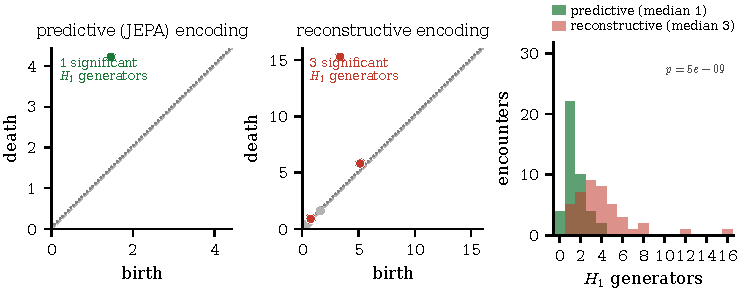
\includegraphics[width=0.98\linewidth]{sections/figures/results/fig_persistence.pdf}
  \caption{Persistent homology of the latent encounter on test\_b. Left and
  centre: representative Vietoris--Rips $H_1$ persistence diagrams of the
  simulation-encoded predictive and reconstructive latents; coloured points are
  significant generators (lifetime above the dotted noise floor) and grey points
  are noise. Right: the distribution of the significant-$H_1$ generator count over
  the $42$ held-out encounters, the scale-free signal. The unconditioned predictive
  encoding is a single clean loop (median one generator) while the reconstructive
  encoding fragments (median three to four; Mann--Whitney one-sided
  $p = 4.9\times10^{-9}$).}
  \label{fig:persistence}
\end{figure}

The third test makes the geometry physical by comparing latent distances with the
unbalanced optimal-transport distance between vorticity fields. Euclidean distance
between vorticity
fields is insensitive to the spatial transport of structures, whereas an
unbalanced optimal-transport (OT) distance measures the cost of rearranging one
field into another and so tracks advection of the LEV and shear layer
\citep{tran2026}. Computing the OT distance between simulation fields along an
encounter gives a physical transport geometry against which the latent metric
can be checked: the prediction is that distances in the predictive latent track
the OT distances more faithfully than distances in the reconstructive latent, so
that iterating the predictor step keeps the rollout closer to the data manifold.
The
prediction holds: the per-encounter Spearman correlation between the latent
distance matrix and the simulation OT-distance matrix on test\_b is $0.61$ for
the predictive latent against $0.45$ for the reconstructive latent, a margin of
$0.16$. The predictive latent metric is therefore more aligned with the physical
transport geometry, in this empirical distance-matrix sense, consistent with a
rollout that remains closer to the encoded manifold. We report this per encounter
rather than pooled across encounters, and we are explicit that the statistic is
trajectory-local: pooling across encounters conflates the within-encounter geometry
with a between-encounter latent-norm scale that the drift-prone reconstructive
latent inflates, which reverses the pooled statistic ($0.41$ predictive against
$0.63$ reconstructive) and is itself a symptom of the same drift. We therefore claim
trajectory-local transport consistency, not a global isometry.

\subsection{Where the wake is kept and where it is lost in physical space}
\label{sec:res_param_phase}
\label{sec:res_physical}

The mechanism explains why the predictive rollout stays on the manifold; we now
ask where in the gust envelope, and where in the flow field, the latent keeps the
wake. The parameter dependence reveals one clear weakness, and it is worth noting
that the latent encodes these parameters despite never being trained on them.
Probing the predictive latent for the gust parameters on test\_b recovers the gust
strength $G$ and the core diameter $D$ ($R^2 = 0.46$ and $0.80$) but barely resolves
the wall-normal offset $Y$ ($R^2 = 0.10$). This is a property of the data rather than of the
architecture: the training mass concentrates near $Y \approx 0$, so encounters
at different offsets within the envelope are weakly separated along $Y$, and the
latent inherits that weakness. Any deployment-time parameter estimate should
treat $Y$ as a nuisance variable the encoder resolves only weakly.

The same latent can also be read relative to the undisturbed shedding cycle.
Because the undisturbed wake
is a limit cycle (\S\ref{sec:flow_physics}), an encounter is naturally described
by its phase and amplitude relative to that cycle, the same reduction used to
design gust-mitigation control for these flows \citep{fukami2024control}. Reading
the predictive latent this way makes ``recovery'' precise: it is the return of
the latent trajectory to the baseline limit cycle. The predictive latent of the
undisturbed case does trace a closed periodic orbit
(figure~\ref{fig:phase_amplitude}): concatenating the four no-gust episodes, the
return distance is $1.0\%$ of the orbit diameter, and the four episodes overlap
the same loop, with a shedding period of about $56$ frames ($2.8$ convective
times, Strouhal number near $0.36$). A phase advances monotonically along it
(via the Hilbert analytic signal of the two leading latent principal components),
though the orbit lives in more than two dimensions, so the phase is a reduction
rather than a complete coordinate. A gust encounter departs this orbit and is
carried back toward it under the predictive rollout while the reconstructive
rollout departs further: the median return-to-orbit distance on test\_b is
smaller for the predictive latent at every horizon, and the separation is
bootstrap-robust at $H = 64$ (predictive $8.70$ versus reconstructive $9.96$,
$95\%$ confidence interval on the paired difference $[1.13, 3.25]$), marginal at
$H = 32$. One caveat applies: the simulation gust
trajectories do not themselves fully return to the baseline orbit within the
$120$-frame window. That window is the gust-release period itself
($6\,t/c$ at $\Delta t = 0.05\,t/c$, with impact near $2\,t/c$), so only about
$4\,t/c$ of post-impact relaxation is ever observed before the next gust is
released, short of a full return; this is a window-length limitation set by the
gust-release cadence, and at fixed core diameter it is not strength-dependent.
The comparison therefore measures the relative drift direction (the predictive
rollout contracts toward the orbit, the reconstructive one expands away), not a
completed physical recovery. The result is the same at $d = 32$.
This limit cycle and the persistent cycle of the previous subsection are the same
object viewed dynamically and topologically.
\begin{figure}
  \centering
  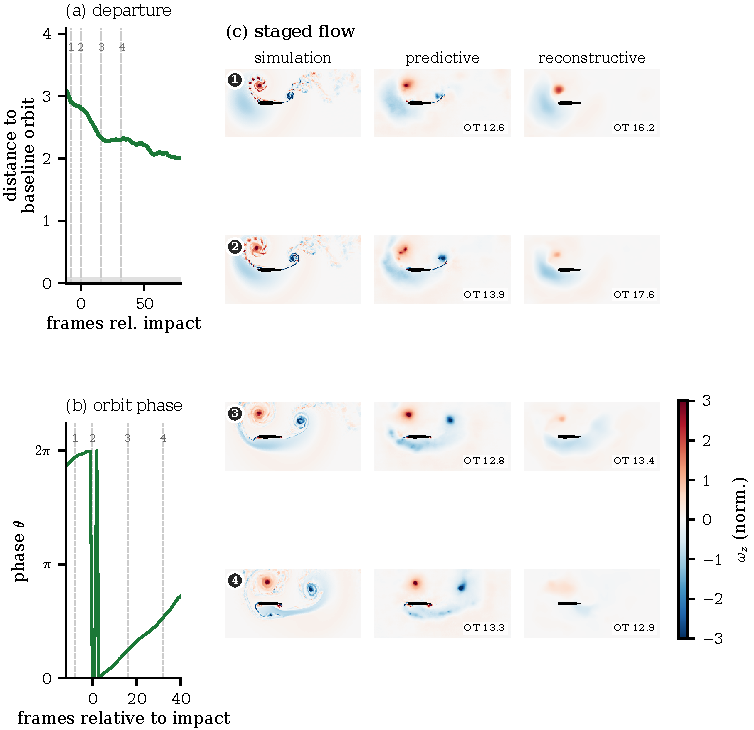
\includegraphics[width=\linewidth]{sections/figures/results/figC_cycle.pdf}
  \caption{The gust encounter in the predictive latent, for a strong negative
  gust $(G, D, Y) = (-3.0, 1.5, -0.1)$. (a) Distance of the gust trajectory to the
  baseline orbit (full latent, in units of the orbit diameter; the grey band is
  the baseline orbit thickness): the encounter departs the baseline cycle and only
  partially relaxes back, without closing within the inter-gust window;
  the single-cycle topology of the encoded latent
  is established coordinate-free in figure~\ref{fig:persistence}. (b) The orbit
  phase relative to the impact frame. (c) Mid-plane vorticity at the four stages
  (rows) for the simulation, the predictive decode, and the reconstructive decode
  (columns); the predictive decode localises the impingement while the
  reconstructive decode collapses, with the optimal-transport field distance
  between each decode and the simulation annotated at each stage (largest for the
  reconstructive decode near impact). The numbered stages are those of
  figure~\ref{fig:traces}.}
  \label{fig:phase_amplitude}
\end{figure}

We can also locate where in the envelope the predictive advantage concentrates.
Rather than a
per-stratum closure table, which the present test set is too small to populate,
we read the per-encounter paired improvement
$\Delta e = e_{\text{AE}} - e_{\text{JEPA}}$ in held-out wake-enstrophy error
directly against each gust axis with a locally weighted regression and a
bootstrapped band (figure~\ref{fig:error_maps}). The advantage is not uniform
across the envelope. It grows with the gust core diameter $D$ (Spearman
$\rho = 0.42$ on the encoded latent, $0.53$ under forecast) and toward
off-midplane wall-normal offset $Y$ ($\rho = 0.49$ and $0.45$), both significant,
while its dependence on the gust strength $G$ is weak on the encoded latent and
moderate under forecast. The predictive advantage therefore concentrates away
from the $Y \approx 0$ training mass and at the larger cores that most reorganise
the wake, consistent with the weak $Y$ resolution of the probe above. The
shedding phase at impact, the axis the gust-response literature emphasises
\citep{fukami2024control}, is only weakly sampled by this dataset: impact is fixed
near a single convective instant while the gust recurs about every two shedding
periods, so the encounters fall into essentially two phase clusters and a
phase-resolved trend is not identifiable here, which a design that varies the
impact phase would isolate.
\begin{figure}
  \centering
  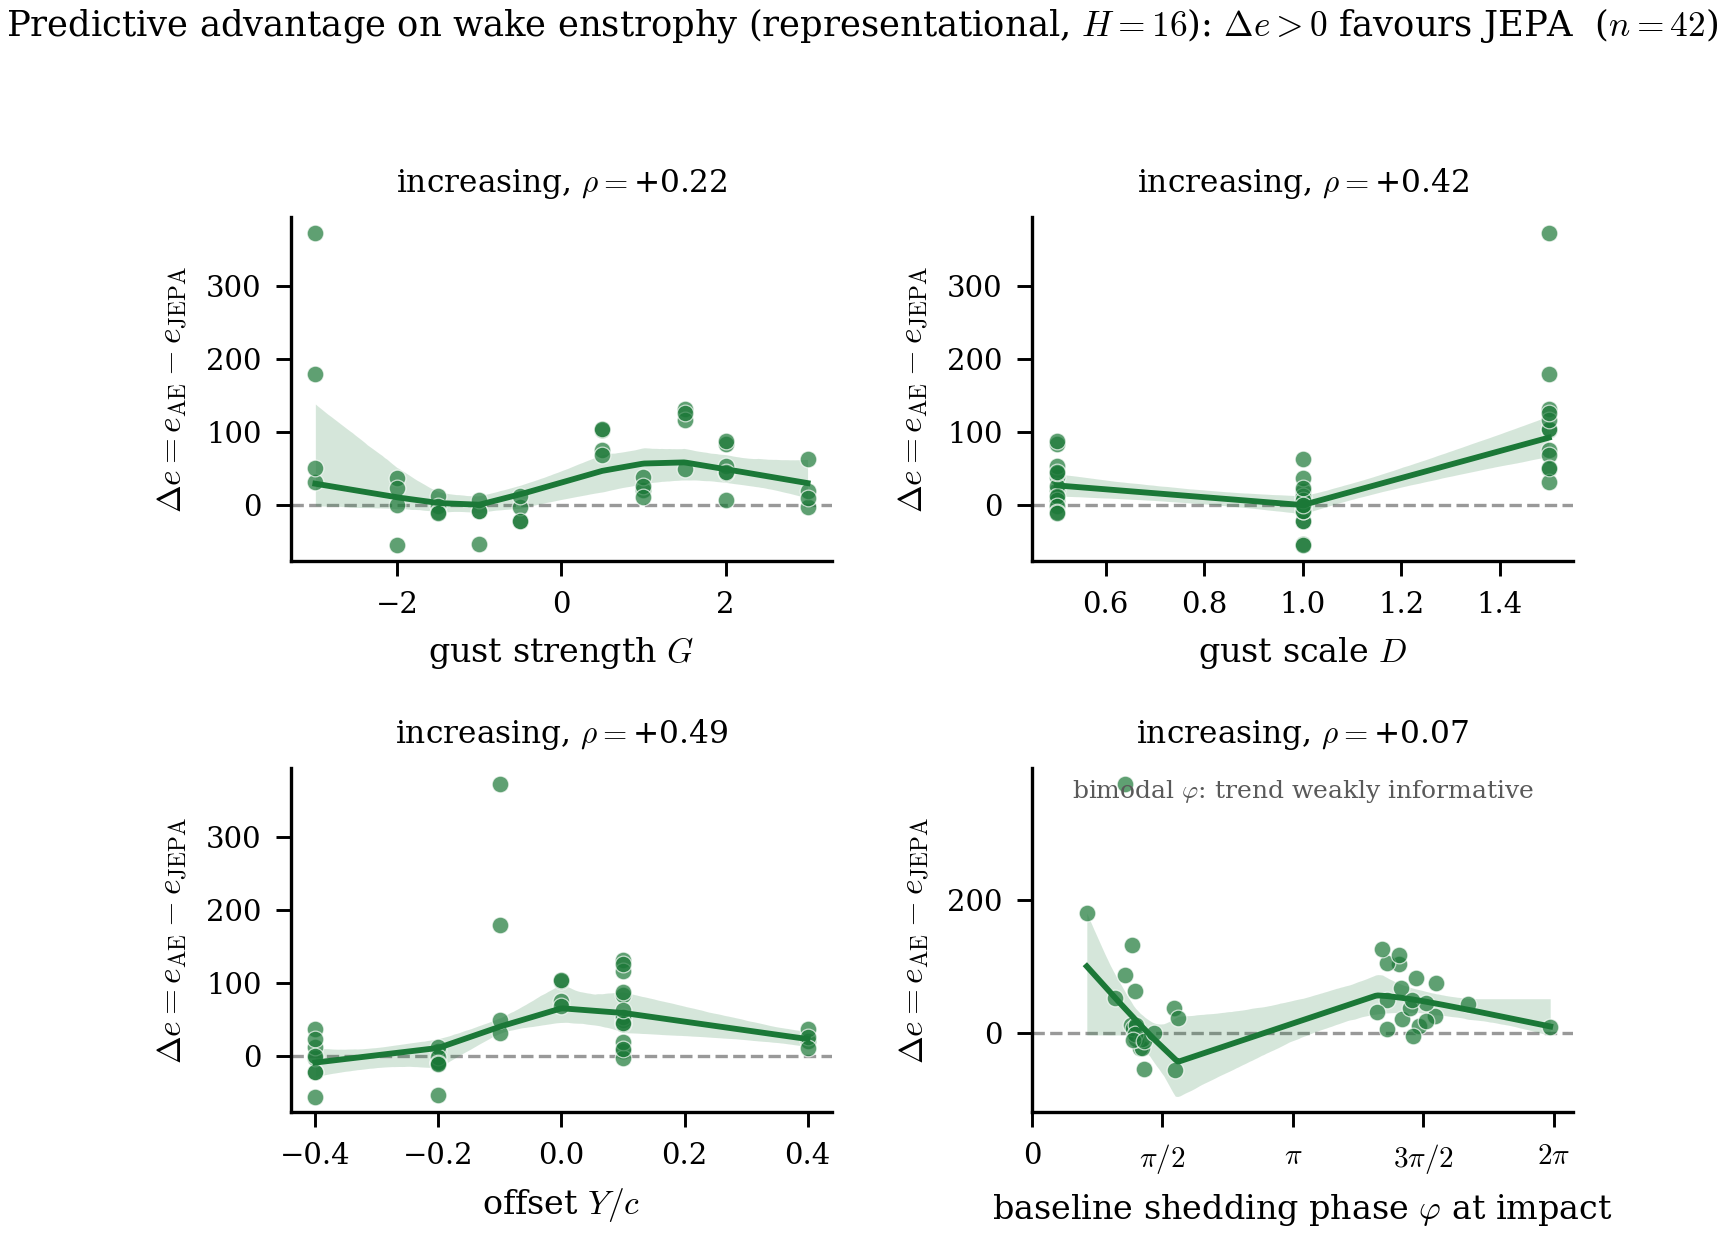
\includegraphics[width=\linewidth]{sections/figures/results/fig_error_maps.png}
  \caption{Per-encounter paired improvement
  $\Delta e = e_{\text{AE}} - e_{\text{JEPA}}$ in held-out wake-enstrophy error
  against the gust strength $G$, core diameter $D$, wall-normal offset $Y$, and
  the baseline shedding phase at impact $\phi$ (test\_b, $n = 42$); positive
  $\Delta e$ means the predictive latent carries the smaller error. Each panel
  shows the per-encounter values, a locally weighted (LOWESS) trend, and a
  bootstrap band over encounters. The predictive advantage grows with $D$ and
  toward off-midplane $Y$; the shedding-phase axis falls into two clusters because
  impact is fixed near a single convective instant.}
  \label{fig:error_maps}
\end{figure}

These parameter and phase readings are statements about numbers; the encounter is
itself a statement about
vortices. Decoded and reconstructed vorticity fields on held-out encounters
(figure~\ref{fig:recon}) connect the two, with one
methodological caution and one new metric. Two scoping points apply throughout
this subsection. The fields are encode-decode reconstructions, the visualisation
decoder applied to the simulation-encoded latent, so the quantitative comparisons
report the decoder's ceiling on what each latent carries from a faithfully encoded
field, not a forecast rollout, whose latent leaves the data manifold for the
reconstructive baseline (\S\ref{sec:res_drift}). And every quantitative
physical-space claim is made on the validated large-scale band ($\sigma/c = 0.05$);
the visualisation decoder is blurry at small scale by construction, so the
large-scale leading-edge vortex and shear layer are tracked meaningfully while
full-resolution and small-scale field fidelity are not claimed.

\begin{figure}
  \centering
  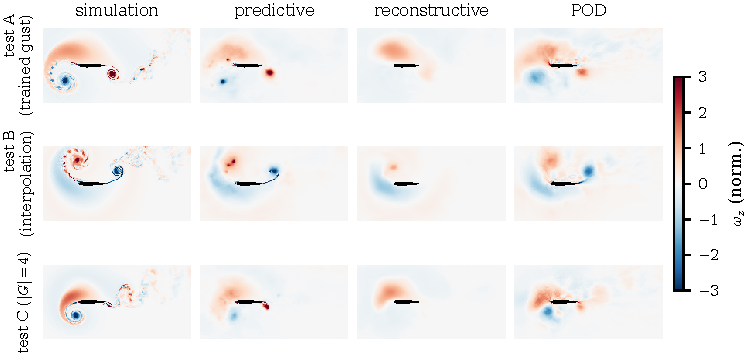
\includegraphics[width=\linewidth]{sections/figures/results/figD_reconstructions.pdf}
  \caption{Decoded vorticity at the impact frame on held-out encounters from the
  three splits (rows: a trained-gust test\_a encounter, an interpolation test\_b
  encounter, and a $|G| = 4$ test\_c encounter) for the simulation and the
  predictive, reconstructive, and POD decodes (columns). The predictive decoder is
  blurry by design but localises the impingement; the reconstructive autoencoder
  collapses toward a near-uniform field on the held-out interpolation condition,
  while the linear basis is amplitude-accurate. All families degrade in the
  $|G| = 4$ regime, reported as the observability boundary of
  \S\ref{sec:flow_physics} rather than as a generalisation claim. Field-space
  similarity is reframed by the optimal-transport metric introduced below.}
  \label{fig:recon}
\end{figure}

The caution is that field-space similarity scores are misleading here. On a
held-out interpolation encounter the reconstructive autoencoder attains a high
structural similarity yet a peak reconstructed vorticity magnitude of only
$0.36$ against a target peak near $9.7$: it has collapsed to a near-uniform mean
field and lost the vortex-impingement signature, and the high similarity merely
reflects bulk agreement with a field that is itself mostly quiescent away from
the impact region. The predictive latent localises the impingement at the right
position and sign (peak magnitude $5.31$) but its visualisation decoder is blurry
by construction, and the linear basis is amplitude-accurate (peak $4.10$) since
its objective is amplitude-optimal.

The new metric resolves the caution. An unbalanced optimal-transport distance
between the reconstructed and the simulation fields, computed for the positive
and negative vorticity separately and summed \citep{tran2026}
(entropic unbalanced Sinkhorn transport cost with a KL marginal relaxation, fields pooled to $48 \times 24$ for tractability),
penalises the collapsed reconstruction correctly and reorders the comparison
where structural similarity misleads (figure~\ref{fig:ot}). At the impact frame
on test\_b the transport distance is largest for the reconstructive autoencoder
($11.25$) and smaller and comparable for the predictive decode ($9.90$) and the
linear basis ($9.95$). The instructive case is the linear basis: it carries the
\emph{highest} structural similarity of the three ($0.69$ against $0.65$ for the
predictive decode), which would wrongly crown the energy-optimal reconstruction
as the best, yet under transport it is no better than the blurry predictive
decode and far better than the collapsed autoencoder, which is the physically
correct ordering. We therefore lead with the transport distance and report
similarity alongside for continuity. On the OOD test\_c set
($G = +4$) the transport ordering breaks (the reconstructive distance falls below
the predictive one), so the transport advantage is an in-envelope result, of a
piece with the three-dimensional observability boundary that degrades every
metric there.
\begin{figure}
  \centering
  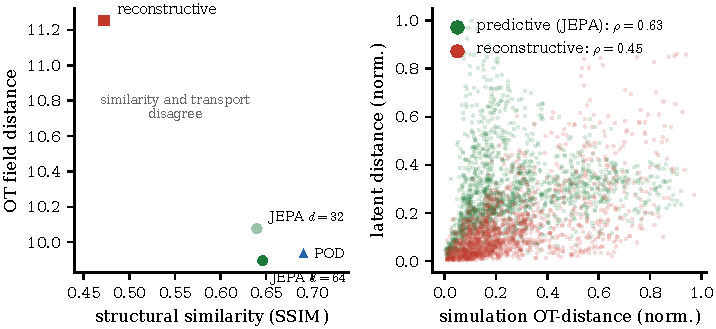
\includegraphics[width=0.9\linewidth]{sections/figures/results/fig_ot.pdf}
  \caption{Optimal-transport reconstruction comparison (Tran et al., JFM 2026)
  on test\_b. Unbalanced OT field distance by family at the impact frame, with the
  structural-similarity ranking shown alongside; the linear basis has the highest
  similarity but no transport advantage over the predictive decode, while the
  collapsed reconstructive field is correctly penalised. The Shepard panel shows
  the per-encounter alignment of latent distance with the simulation
  OT distance, predictive versus reconstructive.}
  \label{fig:ot}
\end{figure}

Finally, the wake observables tie to the structures that carry the load. A
Gaussian scale decomposition (large scale at filter width $\sigma/c = 0.05$,
following \citep{odaka2026,motoori2019}) separates the large-scale vortical
structures responsible for the lift peaks from the fine scale, applied to the
simulation field and to each family's reconstruction
(figure~\ref{fig:scale_decomp}). On test\_b the large-scale wake enstrophy of the
predictive reconstruction tracks the simulation closely (Pearson correlation
$0.89$ at impact and $0.91$ at $H = 16$, relative error $0.22$), while the
reconstructive autoencoder collapses it (correlation $0.23$ and $0.61$, relative
error near $0.8$, retaining only $16$ to $20\%$ of the large-scale amplitude and
almost none of the small-scale energy): it smooths the leading-edge vortex and
shear layer away. The linear basis has comparable large-scale correlation to the
predictive latent but worse amplitude (relative error $0.34$ to $0.38$), so the
claim is specific: the predictive latent tracks the simulation's large-scale
wake structure better than the reconstructive autoencoder on both correlation and
amplitude, and better than the linear basis on amplitude. Across the staged
encounter the simulation large-scale enstrophy rises from the gust-induced
leading-edge flux through the LEV roll-up and peak-load shedding; the predictive
reconstruction follows that rise while the reconstructive one stays flat. This is
where the wake-enstrophy advantage of \S\ref{sec:res_closure} becomes a statement
about the leading-edge vortex and shear layer rather than about a scalar.
Tracking the large-scale leading-edge vortex directly makes this quantitative.
Extracting the dominant suction-side vortex from the same $\sigma/c = 0.05$
field, the predictive decode places a coherent leading-edge vortex in all $42$
held-out encounters at $H = 16$, within $0.32$ chords of the simulation centroid
and recovering its circulation to within $5\%$, whereas the reconstructive decode
has smoothed the vortex below detection in $36$ of the $42$ (its large-scale
leading-edge amplitude falls to about a tenth of the simulation), and where it
survives its circulation error is six times larger. Per encounter the
wake-enstrophy error and the leading-edge-vortex circulation error co-vary
(Spearman $0.57$), so the scalar wake observable stands in for the position and
strength of the leading-edge vortex that produces the lift transient. The
result holds at $d = 32$; on the OOD test\_c set the predictive tracking degrades
($0.91$ to $0.65$ from impact to $H = 16$), as expected where the flow becomes
three-dimensional and the mid-plane decomposition is itself incomplete
(\S\ref{sec:flow_physics}).
\begin{figure}
  \centering
  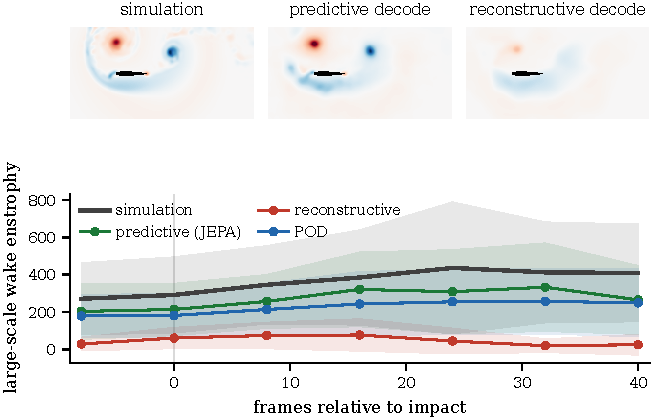
\includegraphics[width=0.98\linewidth]{sections/figures/results/fig_scale_decomp.pdf}
  \caption{Gaussian scale decomposition ($\sigma/c = 0.05$) of the held-out
  reconstructions. Top: large-scale vorticity for the simulation, the predictive
  decode, and the reconstructive autoencoder at $H = 16$; the predictive latent
  retains the leading-edge vortex and shear layer the reconstructive one smooths
  away. Bottom: large-scale wake enstrophy through the staged encounter for the
  simulation, predictive, and reconstructive fields, on each split.}
  \label{fig:scale_decomp}
\end{figure}

\subsection{Wall-pressure observability}
\label{sec:res_observability}

At deployment the vorticity field is not available; only the wall pressure is.
The representational result has an exact deployment mirror: we ask which
representation is most recoverable from a sparse set of $K$ wall-pressure taps over
a pre-impact window, using one kernel-ridge estimator across families for a uniform
comparison (the sensor placement, the lead-time prediction, and a closed-loop pilot
are detailed in Appendix~\ref{app:sensing}). Because the encoder is unconditional in
every case, this observability is unaffected by dropping the gust parameters. The
predictive state is markedly the most recoverable (figure~\ref{fig:observability}a):
with $K = 8$ taps the held-out test\_b state $R^2$ is $0.88$, against $0.58$ for the
reconstructive autoencoder and $0.32$ for the linear basis at $d = 64$, and the
contrast is sharpest at matched capacity. The energy-optimal POD coordinates,
optimal for reconstruction, are the hardest of the three to read from the wall: the
same predictive objective that produces a wake-keeping state produces one that is
also legible from pressure.

Recoverability is not estimation quality, and the distinction is itself
informative (figure~\ref{fig:observability}b). The three-dimensional
reconstructive latent is the \emph{easiest} to recover from pressure (state
$R^2 = 0.91$ at $K = 2$, the highest of any family) yet routing the impact-lift
estimate through it gives the \emph{worst} lift error (mean absolute error $1.0$
against a $C_L$ spread of $1.37$), while the predictive latent gives $0.49$; the
lift itself is read most accurately straight off the pressure ($0.39$), because
the imminent lift is already imprinted on the wall. The contribution of the
predictive latent is therefore the observable, wake-keeping state it carries, not
the instantaneous lift, which is read more accurately straight from the wall.

\begin{figure}
  \centering
  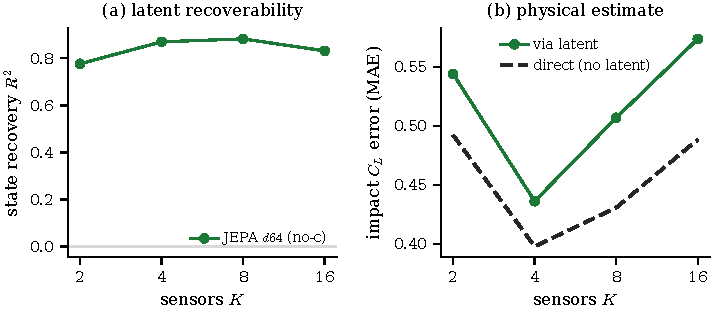
\includegraphics[width=\linewidth]{sections/figures/results/figF_observability.pdf}
  \caption{Cross-family pressure observability under the target-conditioned
  (TCSI) sensor placement. (a) Latent-state recovery $R^2$ versus sensor count
  $K$: the predictive (JEPA) state is the most recoverable at $K \ge 4$, the
  linear basis the least. (b) The physical estimate, impact $C_L$ mean absolute
  error routed through each family's recovered latent, with the direct
  pressure-to-$C_L$ baseline (dashed). The reconstructive $d = 3$ latent is the
  easiest to recover (highest $R^2$ at low $K$) yet gives the worst lift estimate,
  and the lift is read most accurately directly from the pressure.}
  \label{fig:observability}
\end{figure}


\section{Discussion}
\label{sec:discussion}
% Discussion, v3. Restructured around the estimation thesis: 5.1 the design rule
% (division of labour), 5.2 the estimation demonstration and its limits (new),
% 5.3 decodability versus estimability, 5.4 limitations and outlook. Voice per
% the Fukami calibration; every quoted number a macros_v3 macro; the v2.1
% spatial-tier quantitative material and the wake-code figure leave this section
% (the v3 numbers live in Section 4.6; the decode galleries go to Appendix C).
% D244: honest T2b framing, no overselling, Y mentioned only. D243: the merit
% tie is reported as seed-fragile; readability tie robust.
% Session 39 (comparison-led reframe, paper_redesign.md section 5): capacity
% caveat (reviewer risk R3) added to 5.1; the "Choosing the estimator" ladder
% subsection is demotion-bound to the appendix per D-B (flagged inline).

\subsection{What a wall-estimable state must contain}
\label{sec:disc_mechanism}
\label{sec:disc_caveat}

The comparison has a direction, and the deployment ladder of
figure~\ref{fig:deployment_ladder} reads it off. On the decoded field the three
families are indistinguishable, the energy-optimal linear basis as sharp as the
nonlinear states, so field fidelity does not separate them. The separation opens
at the first task that needs the wake, the observable read-out, where the linear
basis loses the load at the impact instant and neither it nor the reconstruction
reads the wake; and it widens at every step toward deployment. Through the impact
the reconstruction's forecast collapses and the linear basis fades; recovering
the state from sparse wall pressure, the predictive latent carries the most
physics from a less recoverable state; and under assimilation at the strong-gust
boundary the predictive filter is the only one that does not diverge on nearly
every encounter. The predictive state is the single family that holds all the way
down the chain, and that is the design rule stated operationally: a state earns
its place at deployment not by rendering the field but by remaining readable,
forecastable, wall-recoverable and assimilable at once.

\begin{figure}
  \centering
  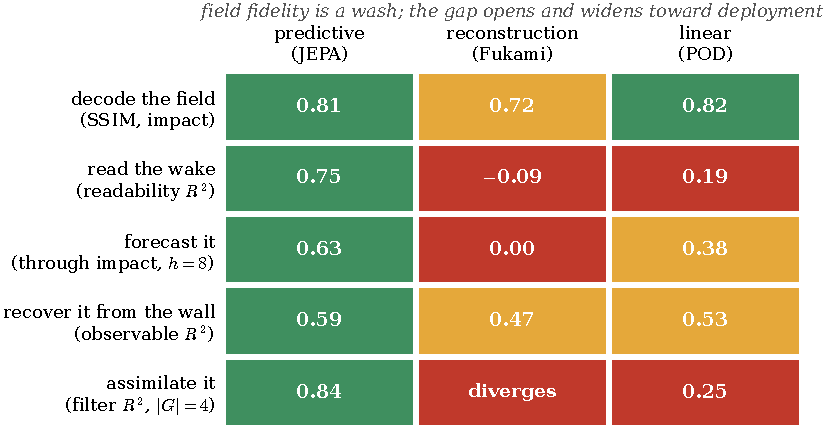
\includegraphics[width=0.92\linewidth]{sections/figures/results/fig_deployment_ladder.pdf}
  \caption{The deployment ladder. Each rung is a task a wall-borne reduced state
  must perform, ordered top to bottom by increasing deployment demand, and each
  cell is the representative metric from the section that establishes it: field
  SSIM at impact (\S\ref{sec:res_compress}), wake readability
  (\S\ref{sec:res_carries}), through-impact forecast merit at $h = 8$
  (\S\ref{sec:res_forecast}), wall observable recovery (\S\ref{sec:res_wallobs})
  and filter closure at the $|G| = 4$ boundary (\S\ref{sec:res_estimation});
  colour marks whether the family holds the rung. Field fidelity does not
  separate the families; the predictive state is the only one that holds every
  rung to deployment. The reconstruction column is the Fukami lineage, its field
  cell the wake-headed variant that alone carries a decoder; at $|G| = 4$ it
  diverges on almost every encounter.}
  \label{fig:deployment_ladder}
\end{figure}

The central result is a design rule for a reduced state that a wall-pressure
estimator can track. Such a state must carry the wake observables that govern the
post-impact transient, must be organised so that a forward model can advance it
without leaving its own support, and must be recoverable from the surface pressure
that is the only measurement a vehicle carries. These three requirements are
supplied by different ingredients, and separating them is the paper's
contribution. Observable supervision on the wake supplies the first, the
instantaneous readability, and, less obviously, much of the second: it
concentrates the encoded variance into a low-rank subspace aligned with the
observables, and the forward rollout, trained and living in that subspace, stays
in distribution, where an anti-collapse regulariser applied to a bare
reconstruction produces a near-isotropic latent with no protected subspace and a
rollout that leaks into the directions the training data never constrained
(\S\ref{sec:res_rollout}). The mechanism is geometric, and it refines our earlier
reading, which credited the anti-collapse term: a reconstruction objective fixes
the latent only up to a diffeomorphism \citep{kelshaw2024}, the anti-collapse term
on its own drives the latent toward isotropy \citep{broustail2026}, and it is the
supervision that pins the variance onto the observable-aligned directions the
rollout respects. The multi-step predictive objective supplies the rest of the
second requirement, the long-horizon stability that a single-step objective and an
objective-free supervised encoder both lack, and, across retrains, the reliability
of the forecast itself (\S\ref{sec:disc_limits}). The third requirement, wall
recoverability, is where energy and information part company: the reconstruction
latent is the most recoverable in raw variance but the least in physics, while the
predictive latent carries the most wall-recoverable physics
(\S\ref{sec:res_wall}), so the coefficient state a controller would want is not
the one a reconstruction objective produces.

The wake, and not the forces, is where these requirements separate the families,
and the coordinate-level reading of \S\ref{sec:res_code} explains why.
The forces are carried redundantly in every family, so an energy or reconstruction
objective retains the force signature of an encounter without retaining the
distributed combination of coordinates that carries the vorticity redistribution
producing it. The gust parameters alone predict the forces well and fail on the
wake at the readout horizon, so a state can look accurate on the load while
carrying none of the physics the load is built from, which is exactly the failure
mode the estimation results expose. The linear basis, for its part, remains
genuinely useful: it is competitive on the body forces, amplitude-accurate in
reconstruction, and it holds the shedding clock as well as the predictive latent
(\S\ref{sec:res_latent_physics}); the result is not that POD is obsolete but that
no linear projection reaches the wake at any dimension we tested.

One caveat is inherited from the compactness-versus-forecast comparison that
motivates this study \citep{solerarico_compactness_underreview}: a more
expressive predictor might narrow the forecast gaps between the families. Three
controls argue that the ordering is a property of the representations rather than
of an underpowered predictor. The shared forecaster was capacity-selected on the
\ValSplit{} set, a sequence-LSTM variant included; the matched autoregressive
transformer diverges on the published-recipe latents at equal recipe and budget,
so its failure is not a capacity artefact; and a per-family tuned recovery
estimator raises every family without changing their order (supplementary
material). The orderings reported here are therefore floors set by the
representation, not ceilings set by the predictor.

\subsection{The estimation demonstration and its limits}
\label{sec:disc_estimation}

The filter turns the design rule into a working estimator: from eight
wall-pressure taps and no field measurement it tracks the load through the
encounter and extends the usable gust-intensity range beyond every static
inverse, realising the online-estimation pathway the extreme-aerodynamic control
literature has named \citep{fukami2024control,mousavi2025,eldredge2025guide}. We
are deliberate about its limits, and the first is one the family comparison
forces: the in-range load-tracking is a property of sequential estimation on a
nonlinear latent generally, not of this state, so the paper does not rest the
representational claim on it. What the predictive state contributes to the
estimator is the strong-gust boundary, the calibration margin, and a tracked
state whose coordinates carry the wake; what no state yet contributes is a
filtered wake estimate, since the analysis wake closure is below the mean
predictor for every family. Its recoverability advantage over a raw
high-dimensional field latent is real but modest (\S\ref{sec:res_wall}), so the
case for the coefficient state rests on the physics-recovery ordering and the
envelope, not on a large recoverability margin. Its point tracking is good but its uncertainty is under-dispersed at the
strongest and widest gusts, where the innovations are temporally correlated and
the ensemble collapses. The visibility analysis suggests the mechanism: the
forward model has large gain along the data-unconstrained near-null directions it
never learned to damp, and those inject spread-consuming noise during
assimilation. This points to a calibrated process and observation noise model,
rather than covariance inflation, as the outstanding requirement, and we report
the filter as a feasibility demonstration with a characterised soft spot, not as a
deployed estimator.

The delay-embedding view names the deployment knob and its limit. Because the
encounter is low-dimensional, the state can be tracked from few taps read over a
short window, which is the sensing budget a small vehicle could carry; the trade
between tap count and window length is explicit for the static reconstruction
(\S\ref{sec:res_delays}), so a sensor-poor platform can in principle compensate
with a longer window within the encounter's own timescale. The frozen filter does
not inherit that trade, because its innovation rank, not the embedding, is what
binds at reduced tap count, and the two statements together sharpen the same
conclusion: the noise model, not the sensor count, is the binding constraint. The
limit that no budget escapes is the growth of the encounter's effective dimension
with gust strength. Read through delay coordinates the encounter is an
intermittently forced low-dimensional system \citep{brunton2017chaos}, the
baseline shedding carrying the delay-coordinate dynamics and the vortex impact
acting as a forcing whose amplitude is the gust ratio, which is consistent with
the envelope being organised by $|G|$: no fixed sensing budget embeds the
strongest, most three-dimensional encounters, which is why the envelope closes
where it does (\S\ref{sec:res_envelope}).

\subsection{Decodability versus estimability}
\label{sec:disc_decode}

A reduced state can be optimised for two deployments that pull apart. A spatially
resolved latent decodes the vorticity field more sharply than the coefficient
state, but it is of far higher dimension than the wall measurement and so is not
recoverable from a sparse set of pressure taps. The coefficient state decodes the
field less sharply and is the object a wall-pressure filter can track. We therefore
separate the two roles: the coefficient state is the estimable, forward-usable
object this paper is about, and the field-resolved latent is a decodability
instrument rather than an estimation target. Pooling the encoder onto the
coefficient state costs field fidelity across every family, by
$\PfourSsimDeltaJepa$ in decode similarity and $\PfourMeritDeltaJepa$ in
fitted-operator forecast merit for the predictive latent (supplementary material),
and it gains nothing in wall recoverability that the coefficient state does not
already have. The state a controller would carry is therefore not the one a
field-reconstruction objective produces.

\subsection{Limitations and outlook}
\label{sec:disc_limits}
\label{sec:disc_control}
\label{sec:disc_outlook}

Five limitations bound the claims. First, the attribution of the instantaneous
results is unglamorous: the wake readability is supplied by the
observable supervision and its tie between the predictive and reconstructive
wake-headed states is seed-robust ($\SeedWakeJepaVec \pm \SeedWakeSdJepaVec$
against $\SeedWakeAeWake \pm \SeedWakeSdAeWake$).
% REVIEW-CLAIM: (Session 36, Track M1, D310) the suited-operator "narrow lead"
% this passage previously cautioned against is gone from the main text; the
% shared-operator recomputation makes the tie explicit, and the earlier U-Net
% seed study now corroborates rather than qualifies it.
The shared-operator forecast merit of \S\ref{sec:res_closure} shows the same
picture dynamically: over three operator seeds the three wake-headed states are
statistically indistinguishable, with overlapping case-clustered intervals. An
earlier seed study of the fitted merit, run under the residual U-Net operator
as a stability check, cautions the same way: the supervised
control is seed-fragile (spread $\SeedMeritSdSupOnly$, with one healthy retrain in
three collapsing), the predictive latent is tighter but not the sharpest
($\pm \SeedMeritSdJepaVec$), and the family means overlap. No fitted-operator
margin between the wake-headed states
is therefore decisive on its own. The defensible dynamical claim rests instead
on the co-trained model and its rollout: the \PredState's own predictor forecasts
better than the shared operator extracts from any latent at short horizon
(\S\ref{sec:res_closure}), and the
multi-step objective confers long-horizon stability and lower drift, not a larger
instantaneous readability margin. Second, the wall-normal offset $Y$ remains the least
resolved release parameter because the training mass concentrates near
$Y \approx 0$; the additional cases make it weakly readable where it was
unreadable before (\S\ref{sec:res_latent_physics}), and we note this without
leaning on it. Third, the $|G| = 4$ extrapolation degrades for a physical reason:
the encoder observes a single mid-plane vorticity slice whose information no
longer determines the three-dimensional dynamics there
(\S\ref{sec:flow_physics}), so the \BoundarySplit{} set marks the observability boundary of that
representation, not a parametric-generalisation claim, and the filter meets the
same boundary from the sensing side (\S\ref{sec:res_envelope}). Fourth, the
visualisation decoder is a diagnostic on the frozen encoder, never part of the
predictive loss, and the pooled coefficient state trades decode sharpness for
estimability by construction (\S\ref{sec:disc_decode}). Fifth, and foremost for
what comes next, the filter's calibration is the priority open problem: its
uncertainty is under-dispersed at the strongest gusts, and the natural next step
is a learned or physically motivated process and observation covariance, ahead of
any closed-loop use.

These limitations come into sharpest focus against the use the architecture is
meant for. The predictor is, by construction, a latent dynamics function of the
kind an estimator or controller requires, the latent is orders of magnitude
cheaper to advance than the field, and the filter demonstrates the estimation half
of that loop from the wall alone. Closed-loop actuation is outside the present
evidence: the predictor is trained to forecast observed encounters within the
training envelope, and predicting how an encounter would differ under intervention
is a task its training does not address. The contribution is narrow by design, a
controlled comparison and a frozen-filter characterisation on a single parametric
flow, and what it establishes is bounded accordingly: a wall-estimable,
forward-usable coefficient state, the ingredients that produce it, and the
gust-intensity envelope over which a fixed sensing budget can follow it. The
natural next steps are the noise model above and the same matched-estimator
protocol on other parametric flows, to test how general the estimability ordering
reported here actually is.


\section{Conclusions}
\label{sec:conclusions}
% Conclusions. Short, in the idiom of the reference papers' "Concluding remarks".

We asked which reduced-order state renders the wake that governs the transient load
linearly readable in parametric vortex-gust airfoil interactions, and reached a
representational answer with a geometric mechanism: a wake-supervised predictive
latent builds a state from which the wake is linearly decodable and whose rollout
stays on the encoded manifold, whereas a reconstruction objective carrying the same
supervision smooths the wake away and its rollout drifts off the manifold along
directions of negligible encoded variance. A control shows the representational
readability is supplied by the wake supervision rather than by the predictive
objective, which is distinguished instead by preserving that readability where
reconstruction suppresses it and by rendering the wake forecastable from the
rollout. We tested this by comparing a predictive
latent (JEPA, which takes no gust parameters), a reconstructive observable-augmented
autoencoder, and a proper orthogonal decomposition basis as reduced states at
$\vRe = 5000$, under a protocol in which a single probe family was held fixed so
that only the encoder varied, judging each first by the representational closure of
the wake. On held-out cases the wake-supervised predictive latent renders the wake
linearly readable where the others do not: its representational wake-enstrophy
$R^2$ is $\NumReprWakeJepaTf$ against the reconstructive and linear baselines at or
below zero, the per-encounter advantage survives the pre-registered encounter-level
multiplicity correction (though not the stricter case-level one), and the gust
parameters alone do not supply the wake state (the parametric floor is negative),
while the linear basis remains most competitive on the integrated impulse. The same
separation appears coordinate-free in the rollout drift and in the topology of the
encoded no-gust limit cycle. The latent also carries the flow's own clocks: its
spectrum recovers the shedding frequency as a marginally stable orbit, the wake
response scales with gust strength, and the gust resets the shedding phase. Rolled
forward, the predictor tracks the encounter, which we show but do not present as a
validated forecast. Because the predictive encoder also differs in architecture and
auxiliary supervision, matched controls attribute the advantage to the predictive
objective trained with wake supervision. The same predictive state is the most
recoverable of the three from sparse wall pressure, so it is both the most
wake-readable and the most wall-recoverable of the three, the property a downstream
estimator would exploit. We do not claim a validated forecast, a controller, or a
counterfactual model. The remaining limitations are the weak resolution of the
wall-normal offset, the three-dimensional observability boundary at $|G| = 4$, and
a rollout error that still prevents a closed-loop control demonstration.


\section*{Funding}
\textit{[Authors to insert funding sources and grant numbers.]}

\section*{Declaration of interests}
The authors report no conflict of interest.

\section*{Data availability statement}
The reduced-order-model and evaluation code, the configuration files, the v2
data-split manifest, and the analysis outputs that regenerate the tables and figures
are deposited at \url{https://doi.org/10.xxxx/zenodo.PLACEHOLDER} under the MIT
License (DOI to be finalised on acceptance). The processed per-encounter cache, or a
representative subset sufficient to rerun the heavier steps, is available from the
corresponding author. The raw direct numerical simulations were computed with the
SOD2D solver \cite{gasparino2024sod2d} and are owned by the simulation
collaborators.

\section*{Author contributions}
\textit{[Authors to insert contributions, for example in CRediT format.]}

\section*{Use of generative-AI tools}
Generative-AI assistance (Anthropic Claude, accessed through the Claude Code
command-line interface) was used during 2026 to help with data analysis, figure
generation, and manuscript drafting. All numerical results were computed by the
authors' own code and verified against the underlying data, and the authors take
full responsibility for the content of the article.

\appendix

\section{Architecture, anti-collapse regularisation, and uncertainty quantification}
\label{app:reg}
% Appendix: architecture detail, anti-collapse regularisation, and uncertainty
% quantification. Describes only what is used on the present (v2) dataset: the
% SIGReg regulariser with its participation-ratio safeguard, and the three
% held-out uncertainty signals. The SIGReg/VICReg/PLDM comparison was a smaller-
% scale development study and is deliberately NOT claimed here.

\subsubsection*{Architecture detail}
The encoder is a hybrid convolutional stem
followed by a small vision transformer. Three downsampling convolutional stages
map the single-channel $192 \times 96$ vorticity field to a $24 \times 12$ feature
map at $256$ channels, that is $288$ spatial tokens, which a six-layer
pre-norm transformer of width $256$ with eight heads processes; the latent is read
from a prepended class token through a one-layer projection whose output passes a
BatchNorm, the layer the characteristic-function regulariser below requires. The
encoder is unconditional and carries no information about the gust parameters. The
predictor is a six-layer autoregressive transformer of width $384$ with sixteen
heads and dropout $0.1$, with a causal mask and rotary temporal positions. The
predictor advances the latent from its own history alone, with no gust input, so
the gust parameters $\cvec = (G, D, Y)$ enter nowhere in the model. Training
minimises the one-step latent prediction loss plus a scheduled-sampling rollout
term and the regulariser below, with AdamW and bf16 mixed precision.

\begin{figure}
  \centering
  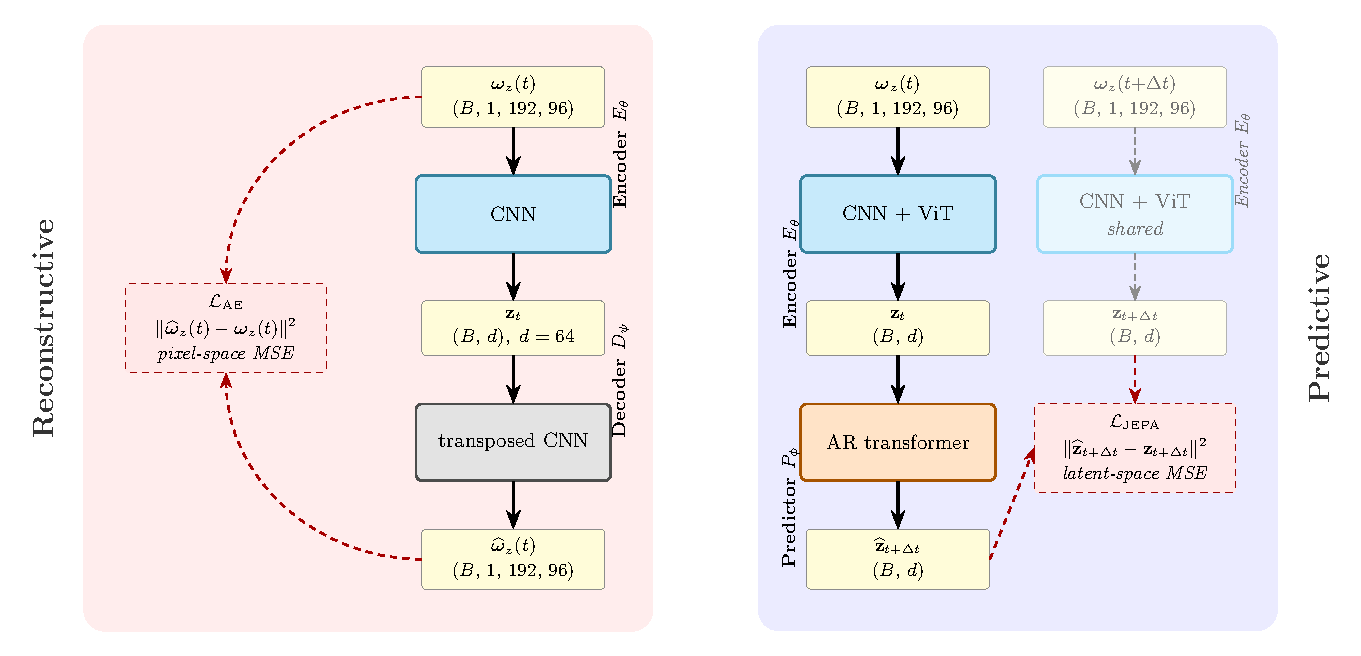
\includegraphics[width=0.95\linewidth]{sections/figures/tikz/fig2_predictive_vs_reconstructive.pdf}
  \caption{Predictive versus reconstructive training. Left: the reconstructive
  autoencoder encodes the field at $t$, decodes it, and incurs a field-space
  error. Right: the predictive model encodes the fields at $t$ and $t+\Delta t$
  with shared weights and incurs a latent-space error between the predicted and
  observed target embeddings, with no field-space loss and no decoder during
  training. This is the contrast the matched-predictor protocol of
  \S\ref{sec:methods_protocol} evaluates; the visualisation decoder is trained
  only afterwards, on the frozen encoder.}
  \label{fig:predictive_vs_reconstructive}
\end{figure}

\subsubsection*{Anti-collapse regularisation}
Because the encoder and predictor are
trained end to end on latent-space prediction with no decoder, the latent is held
away from a collapsed solution by an explicit regulariser rather than by a
reconstruction term. We use SIGReg, the characteristic-function (Epps--Pulley)
regulariser of the from-pixels joint-embedding line \citep{lewm,lejepa}, with $M$
random one-dimensional projections of the latent and a fixed weight
$\lambda_S = \LambdaSigreg$ in the loss, the value used in every run reported
here. The same regulariser has since been adopted independently for biosignal
time series, where it is likewise reported to drive the embedding toward isotropy
so that a structuring objective is needed alongside it \citep{broustail2026},
consistent with the supervision-anisotropy mechanism of
\S\ref{sec:res_rollout}. As a safeguard the participation ratio of the latent is
monitored every thousand iterations, with an automatic fall-back to a
variance-covariance objective \citep{vicreg} if it indicates collapse while the
parameter probe is still uninformative; on the runs reported here the
participation ratio stays healthy and the fall-back does not trigger.

\subsubsection*{Uncertainty quantification}
Every held-out coefficient of
determination and mean absolute error in the paper carries three independent
uncertainty signals, following the reporting protocol fixed with the split. The
first is a bootstrap confidence interval from $2000$ resamples over the held-out
test encounters, which is the dominant source of scatter at the present sample
size ($n = 42$ for test\_b, $n = 24$ for test\_c) and is wide for the individual
wake observables, as noted in \S\ref{sec:res_closure}. The second is the variance
across three encoder retrains from independent random seeds, reported as the
standard deviation in the objective-times-architecture controls of
\S\ref{sec:res_controls}. The third is a five-fold cross-validation over cases on
the read-out (probe) step, which guards against a probe that overfits the
particular held-out split. Together these approximate what a full five-fold
case-level cross-validation of the entire pipeline would buy, at a fraction of the
training cost; a single split with bootstrap intervals is the community standard
for this class of study.

\subsubsection*{Training-set fit}
The predictive latent attains the highest in-distribution training fit of the
forecast rollout among the families, but this is an in-distribution number, not the
held-out result: the family ordering is established by the held-out representational
closure of table~\ref{tab:closure}, and the held-out forecast mean is markedly
lower than the training fit, as it must be. We therefore do not tabulate the
training-set fit, which would invite reading an in-distribution number as a result.

\subsubsection*{Paired tests on the estimation endpoints}
Table~\ref{tab:paired_closure} reports the pre-registered per-encounter paired
family behind the tracking and envelope claims of \S\ref{sec:res_tracking} and
\S\ref{sec:res_envelope}. Pairing cancels the encounter-to-encounter difficulty
that widens marginal intervals, and clustering by case respects the shared
shedding history of a case's encounters.

\begin{table}
  \centering
  \caption{Paired per-encounter tests for the estimation endpoints, on the frozen
  filter records. The family was pre-registered before any statistic was
  computed: the primary family F1 compares the filter analysis against the static
  single-frame recovery and F2 against the field-free open-loop forecast, on the
  endpoints $\{C_L, E_w\}$ in the impact and relaxation windows, one-sided with
  the filter pre-registered as better; $\Delta R^2$ is the median per-case mean
  improvement, the $p$ is a case-level Wilcoxon signed-rank, and Holm corrects
  within each family. On the pooled test\_b encounters the filter beats the
  open-loop forecast decisively on the load but not the static recovery, which is
  accurate at the moderate gust strengths test\_b samples; the filter's advantage
  over the static inverse concentrates at strong gusts, where the test\_c annex
  (characterisation only, $n = \NTestCCases$ cases) is decisive on the load in
  both windows. The wake enstrophy through the filter does not beat the static
  recovery at the boundary, an honest null.}
  \label{tab:paired_closure}
  \small
  \fittab{\begin{tabular}{l l l r l r}
    \toprule
    Family & Endpoint & Window & median $\Delta R^2$ & Wilcoxon $p$ & Holm $p$ \\
    \midrule
    F1 (vs static)    & $C_L$ & impact & $\PsCLImpStMed$ & $\PsCLImpStP$ & $\PsCLImpStHolm$ \\
    F1 (vs static)    & $C_L$ & relax.\ & $\PsCLRelStMed$ & $\PsCLRelStP$ & $\PsCLRelStHolm$ \\
    F1 (vs static)    & $E_w$ & impact & $\PsEwImpStMed$ & $\PsEwImpStP$ & $\PsEwImpStHolm$ \\
    F1 (vs static)    & $E_w$ & relax.\ & $\PsEwRelStMed$ & $\PsEwRelStP$ & $\PsEwRelStHolm$ \\
    \midrule
    F2 (vs open loop) & $C_L$ & impact & $\PsCLImpOlMed$ & $\PsCLImpOlP$ & $\mathbf{\PsCLImpOlHolm}$ \\
    F2 (vs open loop) & $C_L$ & relax.\ & $\PsCLRelOlMed$ & $\PsCLRelOlP$ & $\mathbf{\PsCLRelOlHolm}$ \\
    F2 (vs open loop) & $E_w$ & impact & $\PsEwImpOlMed$ & $\PsEwImpOlP$ & $\PsEwImpOlHolm$ \\
    \midrule
    test\_c annex     & $C_L$ & impact & $\PsCLImpStTcMed$ & $\PsCLImpStTcP$ & -- \\
    test\_c annex     & $C_L$ & relax.\ & $\PsCLRelStTcMed$ & $\PsCLRelStTcP$ & -- \\
    \bottomrule
  \end{tabular}}
\end{table}

\subsubsection*{Topological robustness}
The significant-$H_1$ generator count of
\S\ref{sec:res_drift} declares a generator significant when its persistence exceeds
a noise floor set at a fraction of the cloud diameter (the largest finite $H_0$
death), the canonical analysis using $5\%$ of that diameter and all $120$
trajectory frames. Following the convergence protocol of \citet{smith2024} we sweep
the floor over $\{2, 5, 10, 15, 20\}\%$ and the points per encounter over
$\{120, 60, 40, 30\}$ (uniform subsampling), $20$ settings in all. The predictive
median is one generator in every setting. The predictive-versus-reconstructive
Mann--Whitney separation is below $10^{-3}$ for floors from $2\%$ to $15\%$ at full
($120$-point) sampling and for floors up to $5\%$ at half ($60$-point) sampling
(the canonical $5\%$, $120$-point value is $4.9\times10^{-9}$), while the
reconstructive median falls from six generators at a $2\%$ floor to one at a $20\%$
floor as the aggressive floor filters the spurious generators. Under heavy
subsampling to $30$ points both medians approach one and the separation washes out.
The robust statement is therefore the median-count separation over a defensible
floor and sampling range, not the exact $p$; the case-clustered signed-rank test
($10$ of $10$ cases at the canonical setting) holds across the same range. The full
grid is in the released analysis package.

\subsubsection*{Preprocessing robustness}
The wake enstrophy squares the vorticity, so the per-encounter high-percentile
amplitude clip of the $\omegaz$ preprocessing could in principle shape the primary
endpoint. We test this on the frozen encoders, with no retraining, by recomputing
the readout-frame wake-enstrophy target under three training-only clip treatments of
the raw field and re-fitting the frozen-latent-to-wake ridge probe per family: no
amplitude clip, the production per-encounter $p_{99.99}$ clip, and a single
leak-free $p_{99.99}$ threshold pooled over the training encounters. The predictive
latent leads the wake on test\_b under all three (table~\ref{tab:prepsens}), with
the largest shift in the predictive-minus-best-baseline advantage relative to the
production clip being $\PrepSensMaxShift$ in $R^2$. The leak-free training-global
clip gives the largest predictive advantage, so the per-encounter clip is not the
source of the wake result.

\begin{table}
  \centering
  \caption{Preprocessing robustness of the representational wake closure. Held-out
  test\_b wake-enstrophy $R^2$ at $H = 16$ from a frozen-latent ridge probe (no
  retraining), recomputed under three training-only amplitude-clip treatments of the
  raw $\omegaz$ field. The predictive latent leads the wake under every treatment;
  the advantage keeps its sign and approximate magnitude.}
  \label{tab:prepsens}
  \small
  \begin{tabular}{l c c c}
    \toprule
    Family & no clip & per-encounter & training-global \\
    \midrule
    predictive (JEPA)       & \PrepSensJepaNone   & \PrepSensJepaPerEnc   & \PrepSensJepaGlobal \\
    reconstructive (Fukami) & \PrepSensFukamiNone & \PrepSensFukamiPerEnc & \PrepSensFukamiGlobal \\
    linear (POD)            & \PrepSensPodNone    & \PrepSensPodPerEnc    & \PrepSensPodGlobal \\
    \bottomrule
  \end{tabular}
\end{table}

\subsubsection*{Return to the baseline orbit within the encounter window}
The load-bearing caveat of \S\ref{sec:res_drift}, that the simulation gust
trajectories do not fully return to the baseline orbit within the $120$-frame
encounter, is a consequence of the gust-release cadence rather than a
strength-dependent failure to recover. Figure~\ref{fig:appA_return} holds the
core diameter fixed at $D = 1.0$ with $G < 0$, averages the distance to the
baseline orbit over each case's encounters, and sweeps $|G|$. The departure
amplitude near impact is nearly independent of gust strength (peak distance
$\OrbitReturnPeakMin$ to $\OrbitReturnPeakMax$ orbit diameters across
$|G| \in [0.5, 3.0]$), every trajectory is
still contracting toward the orbit at the end of the window, and the strongest
gust ends closest rather than farthest. The residual offset at the window's end
is therefore set by the $\sim 4\,t/c$ of post-impact relaxation the cadence
allows and by the core diameter, a larger core leaving a more persistent wake,
not by $|G|$. This window-truncated return is common to all three encoders and
does not affect the relative drift comparison of \S\ref{sec:res_drift}, which
contrasts the predictive and reconstructive rollouts over the same window.

\begin{figure}
  \centering
  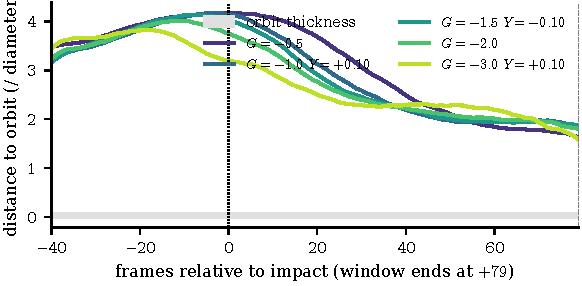
\includegraphics[width=0.82\linewidth]{sections/figures/results/appA_orbit_return_v2p1.pdf}
  \caption{Diameter-controlled return to the baseline orbit. Distance of the
  encoded gust trajectory to the no-gust orbit (predictive latent, in orbit
  diameters; grey band is the orbit thickness), at fixed core diameter $D = 1.0$
  and $G < 0$, averaged over each case's encounters, for five gust strengths. The
  departure amplitude is nearly independent of $|G|$ and all strengths are still
  contracting when the next gust is released at $+79$ frames, so the non-return is
  a window-length effect, not a strength-dependent one.}
  \label{fig:appA_return}
\end{figure}

\subsubsection*{What the latent encodes}
The closure of \S\ref{sec:res_closure} reads single observables at the readout
instant; the latent's broader content is summarised in
figure~\ref{fig:latent_readability}, the held-out $R^2$ of a single linear readout
of the full $64$-dimensional latent to each per-frame flow-state descriptor, on
test\_b, for the three families. The wake-supervised predictive latent is the most
readable on every descriptor: the signed circulations ($\NumLatReadCircPosJepa$
and $\NumLatReadCircNegJepa$), the wake centroid ($\NumLatReadCentroidXJepa$), the
body forces ($C_L$ at $\NumLatReadCliftJepa$), and the wake enstrophy, with the
weakest descriptor still at $\NumLatReadWeakestJepa$. This is a collective property
of the latent, not of any single coordinate: no individual coordinate approaches
the readability of the full latent (the distributed-code gap of
\S\ref{sec:res_code}), and the linear coordinate frame is seed-arbitrary, the
leading subspaces of independent retrains overlapping at the random-rotation level
(squared cosine near $K/d$), so the figure measures how much of each observable is
linearly available in the whole code, not the meaning of any axis. The readout
here pools all post-release frames and is therefore a broader and lower number than
the readout-instant closure: for the wake enstrophy it is $\NumLatReadWakeEnstJepa$
over the full window against $\NumReprWakeJepaTf$ at the impact-plus-$H$ readout,
two regimes of the same encoder rather than a discrepancy. The gust parameters are
omitted because they are an impact-frame quantity (\S\ref{sec:res_param_phase}),
not a per-frame one.

\begin{figure}
  \centering
  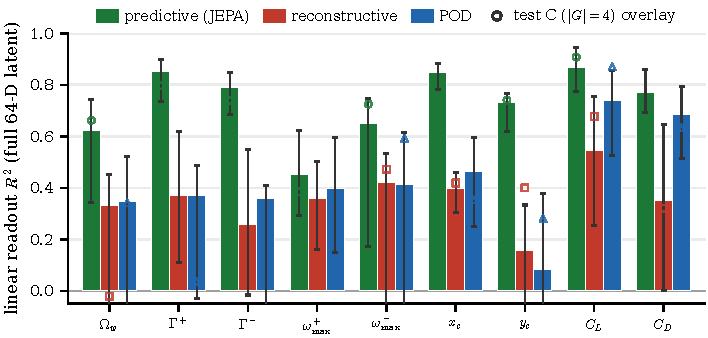
\includegraphics[width=\linewidth]{sections/figures/results/fig_latent_readability_v2p1.pdf}
  \caption{Collective readability of the latent. Held-out test\_b $R^2$ of a single
  linear readout of the full $64$-dimensional latent to each per-frame flow-state
  descriptor, for the predictive (JEPA), reconstructive (Fukami), and linear (POD)
  families; error bars are case-clustered bootstrap $95\%$ intervals and the faint
  open markers are the $|G| = 4$ extrapolation (test\_c). The bars measure how much
  of each descriptor is linearly available in the whole code, not the semantics of
  any individual coordinate; the latent is a distributed representation. The gust
  parameters are omitted as an impact-frame, not a per-frame, quantity.}
  \label{fig:latent_readability}
\end{figure}


\section{Sparse wall-pressure state estimation}
\label{app:sensing}
% Appendix: sparse wall-pressure sensing detail, v3 (Session 33 / D247).
% Rewritten on the v2.2 pooled artifacts (track_o1_recovery, track_t grid,
% envelope + family audit); the previous version carried v2.1 d=64 spatial
% numbers whose recovery ordering CONTRADICTED Section 4.3 (predictive most
% recoverable there; fukami most recoverable here) -- that split-brain is the
% audit finding this rewrite removes. Every number is a macros_v3 macro.

\rb{K}{APB-01}{States the sensing conventions and how the recovery estimator is selected. Needed before any recovery number can be read.}At deployment the vorticity field is not available; only the wall pressure is.
This appendix records the sensing conventions behind \S\ref{sec:res_wall} and
\S\ref{sec:res_tracking} and the placement-robustness checks that the main text
summarises. The input throughout is the span-averaged pressure on the $192$
surface taps; the recovery estimator is selected per family by encounter-grouped
cross-validation among a kernel-ridge regressor on the flattened window, a
multilayer perceptron, and a recurrent network over the window sequence, and the
recovered state is read by the same frozen probes as everywhere else.\re

\subsubsection*{Placement, and why it does not drive the ordering}
\rb{K}{APB-02}{Why the ordering is not an artefact of model-conditioned placement, with the target-blind rerun. Answers a real objection.}Two placements are used, deliberately. The filter and the recovery of
table~\ref{tab:recovery} sense at each family's own model-conditioned taps, the
greedy selection that best exposes that family's latent, because the estimator
comparison should give every family its best sensing. The delay-trade grid of
\S\ref{sec:res_delays} instead uses a single target-blind array, the QR-pivot
optimum of the wall-pressure modes \citep{manohar2018sensors}, nested so that
every tap count is a prefix of the next, because a sensor-budget claim must not
depend on a placement tuned to any model. The two meet where their sensing
coincides: the grid's eight-tap, thirty-frame cell rerun on the
model-conditioned taps closely reproduces the table's recovery
($\TbridgeState$). The energy-versus-information split of \S\ref{sec:res_wall}
is also placement-robust: under the shared target-blind array with the
kernel-ridge estimator alone, the reconstructive state remains the most
recoverable in variance ($\WqStateFukami$ against $\WqStateJepa$ for the
predictive and $\WqStatePod$ for the linear basis) and the predictive state
retains the most recoverable physics ($\WqObsJepa$ against $\WqObsFukami$ and
$\WqObsPod$), so neither ordering is an artefact of the model-conditioned
placement.\re

\subsubsection*{What the window recovers that the instant cannot}
\rb{T}{APB-03}{Restates the window-against-instant result already given in S4-20 and S4-21, with the same macros. The appendix adds only the enstrophy figure.}At a single frame the wall is blind to the wake-circulation direction of the
predictive state (\S\ref{sec:res_wall}); over the thirty-frame window the blind
coordinate becomes partially recoverable ($\ToneCircNegWThirty$ held-out, from
near zero at one frame), and the wake enstrophy read through the recovered state
reaches $\ToneEwWThirty$. The window, not the tap count, is what carries this:
the same quantities barely move as taps are added at a fixed single frame. This
is the delay-coordinate content of the sensing result, quantified in the grid of
\S\ref{sec:res_delays}; it is a statement about the static reconstruction, and
the filter inherits the sequential version of it through its assimilation
window rather than through any explicit delay embedding.\re

\subsubsection*{The recovered field}
\rb{K}{APB-04}{Reads the recovered-field panels and localises the loss to the wake structures. Connects the sensing result to physical space.}Decoding the pressure-recovered state through each family's diagnostic decoder
makes the recovery visible in physical space
(figure~\ref{fig:field_recovery}). The comparison within each row, recovered
field against that family's own decode ceiling, isolates the pressure step from
the decoder's reconstruction limit: the loss from ceiling to recovery is the
part attributable to the eight-tap window, and the panels show it concentrating
in the wake structures rather than in the near-body field, consistent with the
wall reading the force-carrying directions best (\S\ref{sec:res_wall}).\re

\begin{figure}
  \centering
  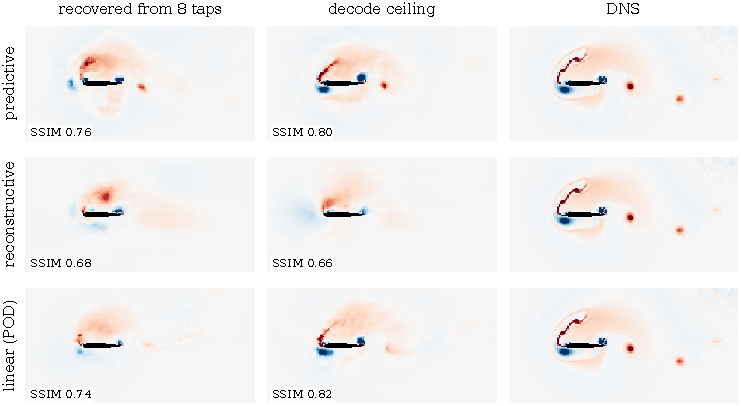
\includegraphics[width=\linewidth]{sections/figures/results/fig_field_recovery_v3.pdf}
  \caption{\rb{K}{APB-C1}{The recovered field against each family's own decode ceiling, which is the only fair comparison. The caption says so.}Flow recovered from eight wall-pressure taps on the representative
  held-out encounter of figure~\ref{fig:hero}, at the impact-side frame, one row
  per family. Columns: the field decoded from the pressure-recovered coefficient
  state, the decode ceiling (the same decoder applied to the encoded state, no
  pressure step), and the simulation; per-panel structural similarity annotated.
  The comparison is within each row, since the decoders' ceilings differ
  (\S\ref{sec:disc_decode}); the ceiling-to-recovered gap is the cost of the
  pressure step.\re}
  \label{fig:field_recovery}
\end{figure}

\subsubsection*{The out-of-distribution boundary from the sensing side}
\rb{T}{APB-05}{Restates the boundary failure of every static approach, already carried by S4-25 and table 12. The appendix repeats the numbers without adding evidence.}At the $|G| = 4$ boundary every static approach fails on the load, the
via-latent recovery at $\VrecCLGFour$ and the direct no-latent regression at
$\DirectCLKeightGFour$ from the same taps ($\DirectCLAllTapsGFour$ with the full
array), while the nonlinear filters still track it (table~\ref{tab:family_filter}). The
boundary is the same larger three-dimensional content the field carries there
(\S\ref{sec:flow_physics}): the mid-plane state captures less of the dynamics, so
a \StaticInv{} recovers little from a single instant, and only the accumulated
pressure history carries the load through.\re

\subsubsection*{Delay-coordinate knobs}
\rb{K}{APB-06}{Justifies the delay stride and window as convention rather than tuning, and declines the false-nearest-neighbours criterion honestly. Methodologically careful.}The window sweeps of \S\ref{sec:res_delays} keep the delay stride at the cache
cadence ($\Delta t = \DtTc\,c/u_\infty$), and this choice is a convention rather
than a tuning: the first minimum of the time-lagged mutual information of the
tap signals \citep{fraser1986} sits near $\TmiTau$ frames, about one shedding
period, so the thirty-frame window spans roughly one decorrelation time of the
wall pressure at the cadence used. The window length itself is selected by the
measured recovery trade rather than by a false-nearest-neighbours criterion
\citep{kennel1992}, which we regard as a cross-check and not a design input: the
delay-embedding guarantees are generic, wall pressure is a physical and
non-generic observable strongly coupled to the near-body vorticity, and the
operative evidence is the measured recovery, with the theorem as the organising
principle rather than a proof that a given tap count suffices.\re

\subsubsection*{Streaming deployment realism and the four-coefficient filter}

% Moved from Results (Session 39, D-B): the streaming realism and d=4 filter
% panels leave the main text with the estimator ladder.
\rb{K}{APB-07}{The streaming realism protocol and the four-coefficient filter, both demoted from \S4.6. Real results, correctly placed.}Under a deployment-realism protocol, streaming multi-encounter assimilation with
a pressure-only initialisation and no oracle anywhere, the filter on the
\PredState{} holds an impact-phase lift closure of \PoneStreamCleanZero{} on
clean taps and \PoneStreamCleanFive, \PoneStreamCleanTen{} and
\PoneStreamCleanTwenty{} at five, ten and twenty per cent tap noise (three
member-noise seeds each, figure~\ref{fig:deploy}). The four-dimensional
lift-critical state of \S\ref{sec:res_dimension} supports a filter of its
own at \PoneDFourFilterImpact{} impact median over five seeds, so a
four-coefficient state is estimable from the wall as well as forecastable.\re

\begin{figure}
  \centering
  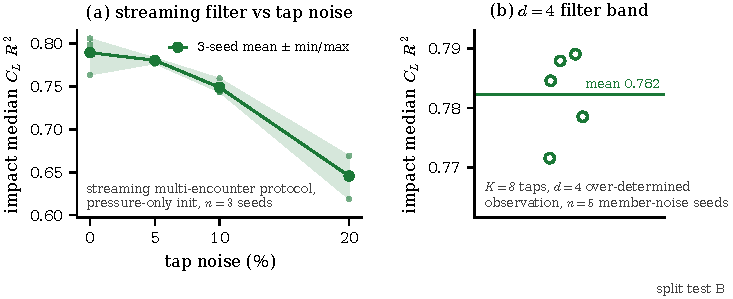
\includegraphics[width=0.9\linewidth]{sections/figures/results/fig_deployment_v4.pdf}
  \caption{\rb{K}{APB-C2}{The deployment-realism panels with the seed counts. Self-contained.}Deployment realism (\TestSplit{} set): (a)~streaming multi-encounter
  filter against tap noise, three member-noise seeds, validation-selected
  band (no test-set reference);
  (b)~the $d = 4$ filter band over five member-noise seeds.\re}
  \label{fig:deploy}
\end{figure}

% Moved from Results (Session 39, figure pass): the scale-invariance panel is an
% envelope diagnostic; the main-text sentence (\S\ref{sec:res_estimation}) points here.
\begin{figure}
  \centering
  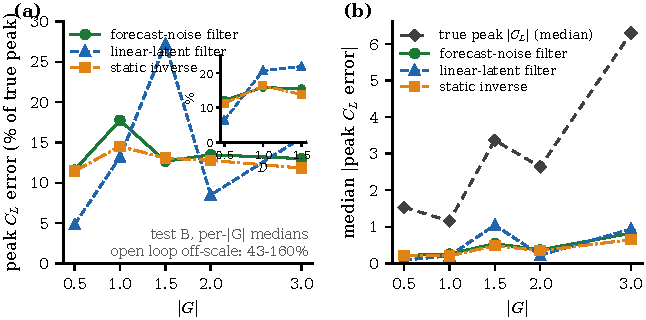
\includegraphics[width=0.9\linewidth]{sections/figures/results/fig_relative_errors_v4.pdf}
  \caption{\rb{K}{APB-C3}{Relative peak error across the envelope, the scale-invariance exhibit \S4.6.3 points at. Self-contained.}Relative peak error across the gust envelope (\TestSplit{} set,
  medians per $|G|$): the forecast-derived filter stays near
  $12$ to $14$ per cent at all but the $|G| = 1$ stratum while the linear
  filter is non-uniform; the
  absolute peak error (right) grows with the peak itself.\re}
  \label{fig:relerr}
\end{figure}

% Moved from Results (Session 39 figure pass): the per-family end-to-end sweeps.
\begin{figure}
  \centering
  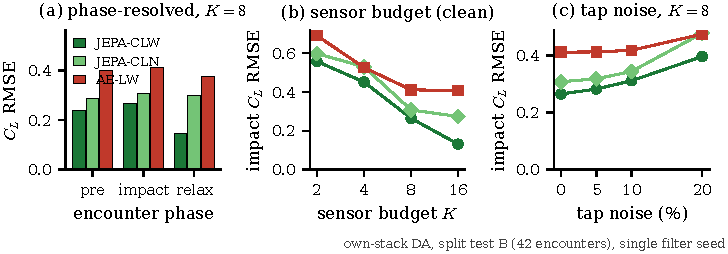
\includegraphics[width=\linewidth]{sections/figures/results/fig_ownstack_da_v4.pdf}
  \caption{\rb{K}{APB-C4}{The per-family end-to-end sweeps behind the own-stack claim. Single-seed provenance disclosed.}Per-family end-to-end comparison (\TestSplit{} set, $42$ encounters,
  single filter seed): (a)~phase-resolved lift error per family;
  (b)~sensor-budget sweep on each family's own nested placement;
  (c)~tap-noise sweep at $K = 8$.\re}
  \label{fig:ownstack}
\end{figure}

\subsubsection*{Choosing among the estimators}
\label{sec:disc_choosing}

% Moved from Discussion (Session 39, D-B): the estimator-selection guidance
% lives with the sensing appendix in the comparison-led revision.
\rb{K}{APB-08}{Explicit estimator-selection guidance in the Gupta idiom, ending in one sentence a practitioner can act on. The most useful paragraph in the appendices.}The ladder of \S\ref{sec:res_da} supports explicit selection guidance
\citep{gupta2026}. When only the in-distribution median matters and latency is
irrelevant, the \StaticInv{} is the strongest and simplest tool; the moment the
tails, the extrapolation boundary or continuous state tracking matter, the filters
take over, the \TwoStageKF{} online and the closed-form fixed-lag smoother on the
linear stack within a quarter-convective-time latency budget, while sparse or
intermittent pressure favours the linear filter with encoded observations (the
only member with zero consistency failures under subsampled updates). Across model
families the guidance is one sentence: anchored latent geometries, predictive or
linear, can be selected on dimension and budget alone, while unanchored
reconstructive geometries require a per-configuration estimatability check that
their probes do not predict.\re


\bibliographystyle{abbrv}
\bibliography{refs,refs_to_add}

\end{document}
